\documentclass{article}

\usepackage{graphics}
\usepackage{amsmath}
\usepackage{amsthm}
\usepackage{amsfonts}

\title{Mixing Enhanced by a Map with Diffusion}
\author{Tzu-Chen Liang}
\date{\today}

% End of Preamble

\newtheorem{example}{Example}
\newtheorem{assumption}{Assumption}
\newtheorem{definition}{Definition}

\begin{document}

\maketitle

\begin{abstract}
   

We study how the mixing of a passive scalar function is enhanced by a map with
diffusion and thus a mixing enhancement factor (MEF) is defined. MEF
is a function of the initial distribution, diffusibility and time.
We discuss both the transient and the long-time tendency of MEF. The
transient MEF is highly related to the well-known cutoff phenomenon
in Markov chain simulation, and the long-time enhancement converges
to a constant which is the spectrum gap ratio of the diffusion
operator and the map with diffusion operator.


\end{abstract}

%%%%%%%%%%%%%%%%%%%%%%
\section{Introduction}
\label{Introduction}
%%%%%%%%%%%%%%%%%%%%%%
The problem of how chaotic advection mixes a passive scalar function has attracted more research efforts in recent years\cite{Ottino2004}. The main issues in this field are: how to measure the thoroughness of the mixing, how to define the efficiency of a mixing process and how to enhance it by designing the map which produces chaotic advection. Unfortunately, we have only fractional understanding on most of these topics.

\paragraph{Measure of Mixing}
There is no consensus on how to measure the mixing of a passive
scalar function so far\cite{Mezic2005}. \cite{Wiggins2004} builds
the hierarchical structure of maps with different mixing properties
qualitatively and characterizes that the most desired mixer has the
property called Bernoulli, but it does not tell anything about how
fast it mixes. Maximum entropy approach has been used in, for
example \cite{DAlessandro1999}, as a measure of mixing. However,
this measure is a property of the dynamical system and independent
of the initial configuration of the scalar function, thus it is not
so useful when one wants to design a mixing protocol for a
particular initial scalar function, and which is quite common in
practice. The simplest and widely used way is to measure the $L^2$
norm or the variance of the scalar function \cite{Ashwin2002},
\cite{Thiffeault2003-13},\cite{Thiffeault2003-309}, []. This
approach can be applied when the mixing process is diffusive or
artificial diffusion is added, otherwise the function is never mixed
in the sense of this measure. This is in general not a problem in
practice because the true system is always diffusive. Nonetheless,
we still want to somehow distinguish the difference between a smooth
scalar function and a highly oscillated one. Clearly $L^2$ norm and
the variance measures are not helpful here. \cite{Mezic2005} defines
a new mix-norm, which resolves this problem and can be served as a
measure of mixing for both diffusive and non-diffusive systems. As
the author stated, this norm is equivalent to the Sobolev norm with
index $s = -\frac{1}{2}$, i.e. it is diagonal in the frequency
domain and weights less on the high wave number terms. So even when
a volume-preserved map is applied to the scalar function, one can
still observe the change of this mix-norm. In fact, any Sobolev norm
with negative $s$ index have this desired property. Hence there are
not much difference in choosing the mix-norm or any of these Sobolev
norm when measuring mixing. In this paper, we will compare these
mixing measures and suggest a more natural one, called
diffusion-norm. Physically, it measures the $L^2$ norm when one
diffuses the scalar function for time duration $t$ and diffusive
rate $D$. The advantage of this measure is for a real system, these
physical parameters actually exist and the mixing in the
corresponding length-scale is the one we care. This diffuse-norm is
also diagonal in frequency domain and decreasing when the wave
number gets higher, so it preserves the property of the mix-norm and
also gives the freedom of adding the important physical quantities
one want to measure.

\paragraph{Cutoff Phenomenon in a Mixing Process}
A widely observed phenomenon in the mixing process is the two or
three-stage transition\cite{Thiffeault2003-13}[][][]. The map does
not mix the scalar function with a constant rate in general. How the
mixing rate changes is also highly dependent of the measure one
uses. The more interesting phenomenon happens when the $L^2$ norm is
applied. One can in general observe a relatively flat decay followed
by a super-exponential change, and then finally it tends to a
exponential decay. Researches are focused on when these transitions
happen and why they happen. \cite{Thiffeault2003-13} studies these
properties for a modified Arnold's cat map. Analytical formulas are
given to predict the transitions as well as the slopes. However, it
is because the linear part of this map stretches very fast (with an
eigenvalue 2.618) and the chaotic part is relatively small so that
the three phases are separated clearly. The same results cannot be
applied to, for example, standard map, although the only difference
between the standard map and the modified Arnold's cat map is in the
linear part. Other physically interpretations are made by [][][] to
explain how the super-exponential decay happen. Nonetheless, it is
also noticed when other norms are applied, this super-exponential
phase may not appear. This suggests that in spite of the richness of
the transient phenomenon is attractive, to answer when it transits
to the exponential decay phase and how the map enhances the decay
rate in this phase are perhaps more important in practice.

A somewhat surprising fact is this two or three-stage transition,
especially the super-exponential decay phase also occurs in some
simple linear systems, and they have been observed and named cutoff
phenomenon in Markov chain simulations. This phenomenon is firstly
found by David Aldous and Persi Diaconis in \cite{Diaconis1986}. The
well-known examples are the birth-death chain[Diaconis2005] and the
riffle shuffle problem\cite{Diaconis1996}, \cite{Diaconis2001}. For
a birth-death chain problem, one can creates a cutoff simply by a
Markov chain system with only several states. As for the riffle
shuffle problem, the number of states is extremely large ($n!$ when
there are $n$ cards). We show this is because the two kinds of
systems are different representations of similar systems, and they
are also close related the chaotic maps. The idea to build this
connection is that we think any chaotic map can be represented as a
infinity dimensional linear system by obtaining the Frobenius-Perron
operator. And then we find the finite dimensional approximation of
this operator to construct a finite dimensional Markov chain. We
then show this Markov chain preserves most of the properties of the
chaotic map with some diffusion. Study of this linear system gives
us the insight of the nonlinear behavior of the chaotic map. For
example, the second largest eigenvalue of this Markov matrix is the
decay rate of the chaotic map with diffusion in the stationary
stage.
\paragraph{Optimization of a Mixing Protocol}
The above approach has yet another great advantage when one wants to
design and optimize a mixing protocol. When designing a mixing
protocol using any of the optimization algorithms, one needs to
obtain a decent direction on which the mixing rate enhances. In a
system represented by a Markov chain, this is corresponding to
minimize the second largest eigenvalue modulus. We will show how a
subgradient direction can be found for the Markov matrix and how it
enables the optimization of mixing channel design when other
constraints, such as the fluid field is physically possible, are
imposed. Numerical simulations are given to demonstrate the
optimized channel.

In the following section, the notations used in this articles are introduced. Section 3 we discuss the different measure of mixing. The method to get a linear approximation of a map is addressed in section 4, and the examples are given in section 5. In section 6 is about the issues to optimize a map, and finally a conclusion is given.






%%%%%%%%%%%%%%%%%%%
\section{Notations}
\label{Notations}
%%%%%%%%%%%%%%%%%%%
\paragraph{Frobenious-Perron Operator}
Let $T^2 =[0,1]\times[0,1]$ be a 2-dimensional torus. We consider
$c:T^2 \rightarrow \mathbb{R}$ to be the density field or the scalar
function. $S:T^2\rightarrow T^2$ is a non-singular (invertible
measure-preserving) transformation, or a map. Then the
Frobenious-Perron operator $[P]:L_{T^2}^2\rightarrow L_{T^2}^2$ is
defined as
\begin{eqnarray}
\label{FPoperator}
  [P]c(\mathbf{x})=c(S^{-1}(\mathbf{x}))
\end{eqnarray}
where $\mathbf{x}=(x,y)$. A continuous-time map $S_c: T^2 \times
\mathbb{R} \rightarrow T^2$ is the coordinate transformation $S_c:
\mathbf{x}_0 \mapsto S_c(\mathbf{x}_0,t) $ for some $\mathbf{x}_0$
and time $t$. Similarly, the continuous-time Frobenious-Perron
operator is written as $[P_c(t)]:L_{T^2}^2\rightarrow L_{T^2}^2$,
which satisfies $[P(t)]c(\mathbf{x}) = c(S_c(\mathbf{x},-t))$.

$[M(D,t)]: L_{T^2}^2  \rightarrow L_{T^2}^2$ is the diffusion
operator, where $D$ and $t$ are the diffusion rate and time. We
define $c'(\mathbf{x}) = [M(D,s)]c(\mathbf{x})$, where
$c'(\mathbf{x})= u(\mathbf{x},s)$ and $u:L_{T^2}^2 \times \mathbb{R}
\rightarrow \mathbb{R} $ is the solution of the following partial
differential equation,
   \begin{eqnarray}
   \label{diffusion equation}
    u_{t} = D(u_{xx}+u_{yy})        \\
    u(x,y,0) = c(x,y)      \nonumber\\
    u(1,y,t) = U(0,y,t)    \nonumber\\
    u(x,1,t) = U(x,0,t)    \nonumber
   \end{eqnarray}
In order to simulate a map with diffusion, we need to solve the
diffusion equation (\ref{diffusion equation}) with a given map. For
a continuous-time map $S_c$, define $v(S_c(\mathbf{x},t),t) =
\frac{d}{dt}S_c(\mathbf{x},t)$ to be the vector field of it. Then
$[P_c(D,t)]:L_{T^2}^2\rightarrow L_{T^2}^2$ is the
map-with-diffusion operator. $c'(\mathbf{x}) =
[P_c(D,s)]c(\mathbf{x})$, where $c'(\mathbf{x})= u(\mathbf{x},s)$ is
the solution of the following PDE at time $s$,
   \begin{eqnarray}
   \label{map with diffusion equation}
    u_{t} + v \cdot \nabla{u}  = D(u_{xx}+u_{yy})        \\
    u(x,y,0) = c(x,y)      \nonumber\\
    u(1,y,t) = U(0,y,t)    \nonumber\\
    u(x,1,t) = U(x,0,t)    \nonumber
   \end{eqnarray}

In discrete-time case, for the time interval $\Delta t$ it is simply
$[P(D,\Delta t)]:L_{T^2}^2\rightarrow L_{T^2}^2$ and
\begin{eqnarray}
\label{PDdef}
 [P(D,\Delta t)]c(\mathbf{x})= [M(k,\Delta t)]c(S^{-1}(\mathbf{x}))
\end{eqnarray}

Define $\sigma: L_{T^2}^2\rightarrow \mathbb{R}$,
\begin{eqnarray}
[\sigma]c(\mathbf{x}) = \left(\int_{T^2}\left(  c(\mathbf{x}) -
\bar{c} \right)^2 da\right)^{\frac{1}{2}}
\end{eqnarray}
where $da = dxdy$ and $\bar{c} =  \frac{\int_{T^2}
c(\mathbf{x})da}{\int_{T^2}da}$ is the mean of $c(\mathbf{x})$ over
$T^2$. $[\sigma]c(\mathbf{x})$ is equal to the $L^2$ norm of the
function $c(\mathbf{x})$ when the mean of $c(\mathbf{x})$ is zero.



$P_h: \mathbb{R}^{1/h^2} \rightarrow \mathbb{R}^{1/h^2} $ and $M_h:
\mathbb{R}^{1/h^2} \rightarrow \mathbb{R}^{1/h^2}$ are the finite
dimensional approximations of Frobenious-Perron and diffusion
operators on regular meshes with size $h$. The same as the operator
$[M(D,t)]$, we use $M_h(D,t)$ to represent the diffusion operator
with diffusion rate $D$ and diffuse time $t$. We also define a
function $[d_h]: T^2 \rightarrow \mathbb{R}^{1/h^2}$ as
\begin{eqnarray}
[d_h]c(\mathbf{x}) = c
\end{eqnarray}
where $c_i = \int_{a_i} c(x,y) da$ for $i = 1,2,...1/h^2$, and $a_i$
stands for the $i_{th}$ grid. So $c$ is the finite dimensional
approximation of $c(\mathbf{x})$ on regular grids with size $h$.


\paragraph{Finite Markov Chains}
Let $\chi$ be a finite space of cardinality $|\chi|=n$. A discrete
time Markov chain is a sequence of $\chi$-valued random variables
$(W_l)_0^{\infty}$ satisfying
\begin{eqnarray*}
 &\mathbf{Prob}(W_l = a_l | W_{l-1} = a_{l-1},W_{l-2} = a_{l-2},...,W_0 = a_0)  \\
 &=\mathbf{Prob}(W_{l} = a_l | W_{l-1} = a_{l-1})
\end{eqnarray*}
for all $a_i \in \chi$ with $0 \le i \le l$ and $l\ge 0$. A Markov
chain is time homogeneous if the quantity in the right hand side
above is independent of $l$. In this case, such a Markov chain is
specified by the initial distribution (the distribution of $W_0$)
and the one-step transition kernal or Markov kernal $K\,:\, \chi
\times \chi \rightarrow [0,1]$, which is defined by
\begin{eqnarray*}
\forall x,y \in \chi, \,\,\, K(x,y)=\mathbf{Prob}(W_{l+1} = y |
W_{l} = x)
\end{eqnarray*}
For any Markov chain $(W_l)_0^{\infty}$ with transition matrix $K$
and initial distribution $w^0$,  $\mathbf{Prob}(W_0=x)=w^0(x)$ for
all $x \in \chi$, the distribution of $W_l$ is given by
\begin{eqnarray}
\label{Kevolvedistribution} \forall x\in \chi \,\,\, w^l(x) =
\mathbf{Prob}\{W_l=x\}=(w^0 K^l)(x)=\sum_{y\in \chi} w^0(y)K^l(y,x)
\end{eqnarray}
where $K^l$ is a matrix defined iteratively by
\begin{eqnarray*}
\forall x,y \in \chi \,\,\, K^l(x,y)=\sum_{z \in
\chi}K^{l-1}(x,z)K(z,y)
\end{eqnarray*}


A Markov kernal $K$ on $\chi$ is said to be irreducible if for any
$x,y$ there exists $j = j(x,y)$ such that $K^j(x,y)>0$. A state
$x\in\chi$ is called aperiodic if $K^l(x,x)>0$ for sufficiently
large $l$, and $K$ is called aperiodic if all states are aperiodic.
Under the assumption of irreducibility of $K$, there exists a unique
stationary distribution $\pi$ satisfying $\pi K =\pi$

If $K$ is irreducible and aperiodic, then
\begin{eqnarray*}
\forall x,y \in \chi \,\,\, \lim_{l \rightarrow \infty}
K^l(x,y)=\pi(y)
\end{eqnarray*}



We work on the ($n$-dimensional) Hilbert space $\ell^2(\pi)$. The
adjoint operator of $K$ is $K^*$,
\begin{eqnarray*}
\label{Kadjoint}
  K^*(x,y) = \pi(y)K(y,x)/\pi(x)
\end{eqnarray*}
$K^*$ is also a Markov operator. The Markov process associated with
$K^*$ is the time reversal of the process associated with $K$. If a
measure $\mu$ has density $f$ with respect to $\pi$, that is, if
$\mu(x)=f(x)\pi(x)$, then $\mu K$ has density $K^*f$ with respect to
$\pi$. Thus acting by $K$ on a measure is equivalent to acting by
$K^*$ on its density with respect to $\pi$.

The above observation says to evolve the density $f$ forward in
time, $K^*$ is the operator one needs, i.e.,
\begin{eqnarray*}
\label{fevolve}
f^l(x) =  (K^*f^{l-1})(x)= \sum_{y \in \chi}
K^*(x,y)f^{l-1}(y)
\end{eqnarray*}
where $f^l$ and $f^{l-1}$ are the densities of $w^l$ and $w^{l-1}$
with respect to $\pi$.





%%%%%%%%%%%%%%%%%%%%%%%%%%%%%%%%%%%%%%%%%
\section{Measure for Mixing}
\label{Measure for Mixing}
%%%%%%%%%%%%%%%%%%%%%%%%%%%%%%%%%%%%%%%%%
In this section we compare the different norms which can be applied
to measure the mixing of a scalar function. The candidates are the
mix-norm suggested by \cite{Mezic2005}, Sobolev norms with index $s
= 0$,$-0.5$, and $-1$, and a diffuse-norm we suggest. All of these
norms are much easier defined in the frequency domain. The
definition of mix-norm can be found in \cite{Mezic2005}. Here the
other norms are given.


For a function $c \in L^{2}_{T^2}$, which has a Fourier
representation $c(\mathbf{x}) = \sum_{k \in \mathbb{Z}^n}
a_\mathbf{k} e^{i 2 \pi \mathbf{k.x}}$, where $\mathbf{k}=
\sqrt{k_1^2+k_2^2}$ and $k_1$ and $k_2$ are the wave number on $x$
and $y$ directions. The Sobolev norm $H^s$ is given by,
\begin{eqnarray}
  \|c\|_{H^s} = \sqrt{\sum_{k \in \mathbb{Z}^n}   \left(1+(2 \pi \|\mathbf{k}\|)^2\right)^s |a_{\mathbf{k}} |^2   }
\end{eqnarray}

The diffuse-norm $\|\cdot\|_D$ is thus
\begin{eqnarray}
  \|c\|_D = \sqrt{\sum_{k \in \mathbb{Z}^n} e^{-4 \pi^2 D \|\mathbf{k}\|^2} |a_{\mathbf{k}} |^2   }
\end{eqnarray}
Physically, the diffuse-norm is equivalent to diffuse the function
$c$ with the diffusion rate $D$ for one unit time step and then
measure the $L^2$ norm. So it can be also written as,
\begin{eqnarray}
  \|c\|_D = \|[M(D,1)] c \|_{H^0}
\end{eqnarray}
Hence all these norms are different only on the coefficient
multiplied by $|a_{\mathbf{k}} |^2$. We thus plot these coefficients
as a function of $\mathbf{k}$ in figure \ref{normcompare}

\centerline{\scalebox{0.5}[0.5]{\includegraphics{normcompare.eps} \label{normcompare}}}

In figures (\ref{normplot}) and (\ref{lognormplot}) we show the
simulations of standard map with the chaotic parameter $\epsilon =
0.2$, diffusivity rate $D = 1e-5$ and initial condition $\mathbf{x}
= cos(x)$. All norms capture the increase of mixing successfully,
whereas the details are different. $L_1$ and $H_0$ (which is just
$L_2$) norms decay super-exponentially and have concave shapes
before iteration $20$. The other norms drop fast in the beginning.
In \cite{Mezic2005} the author claims that the mix-norm is
equivalent to $H_{-\frac{1}{2}}$ norm. This fact is clearly shown in
this simulation. One should also notice that the diffuse-norm has
very similar tendency with the above two norms. This result is not
surprising because in figure \ref{normcompare} they all have
monotonic decreasing weights on high wave numbers.

\centerline{\scalebox{0.5}[0.5]{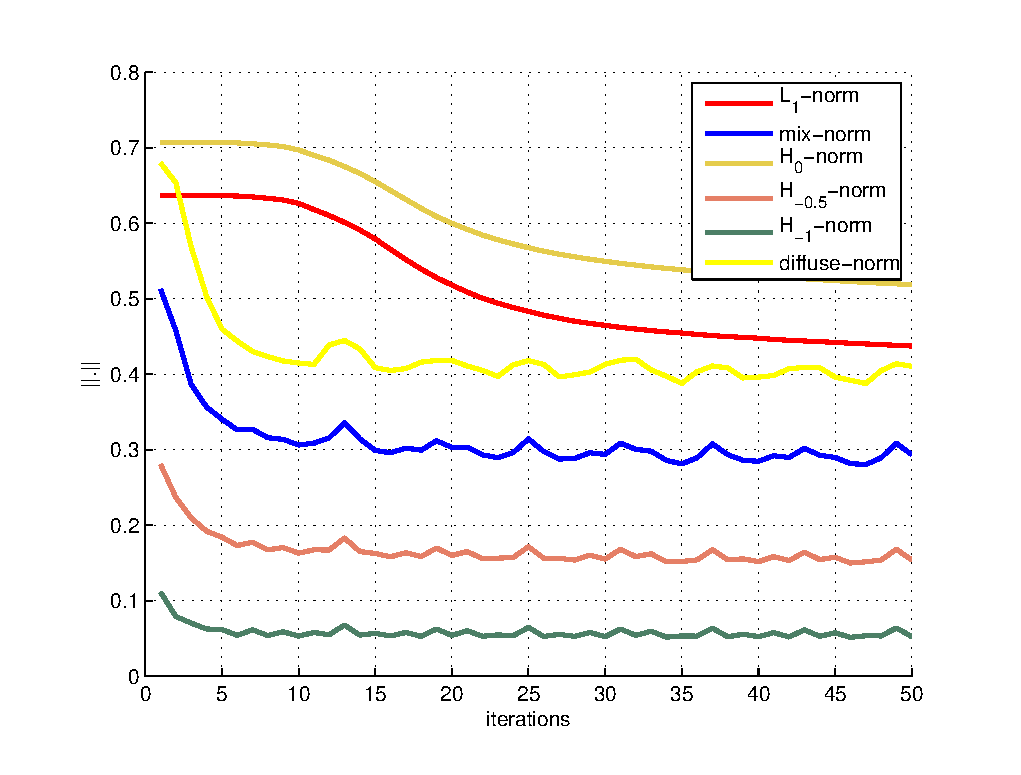
\includegraphics{normplot.eps} \label{normplot}}}
\centerline{\scalebox{0.5}[0.5]{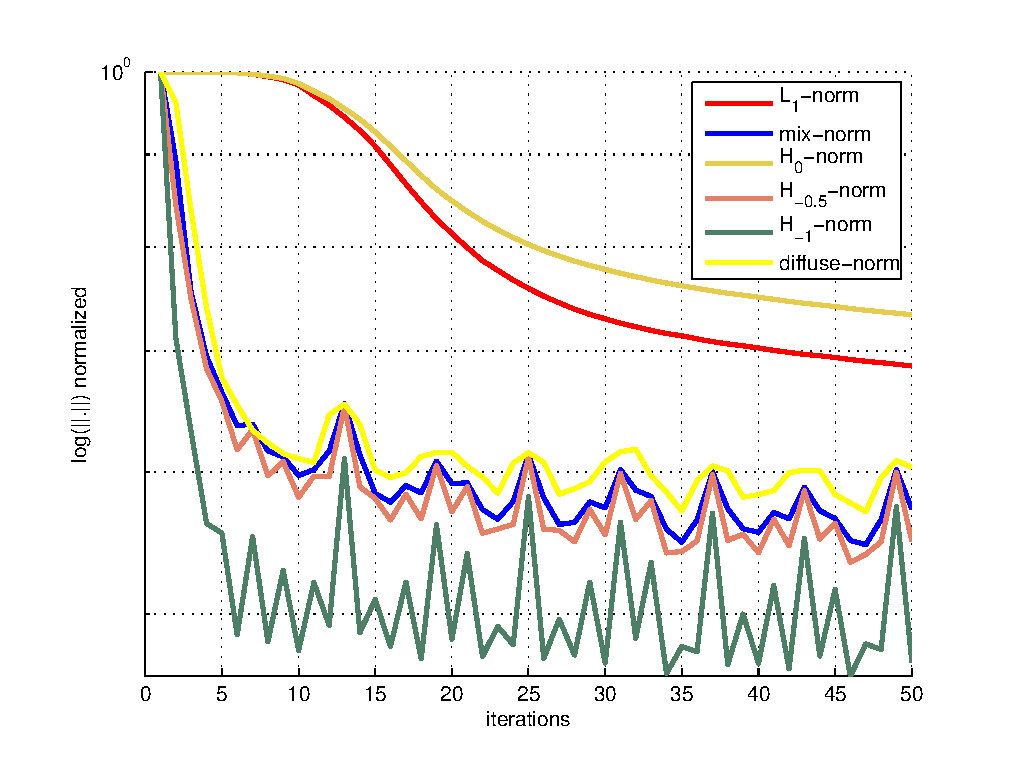
\includegraphics{lognormplot.eps} \label{lognormplot}}}

We think all the norms discussed above are valid for measuring the
chaotic mixing of a scalar function. Which norm one should apply is
dependent of what one cares the most. For example, we can easily
design a norm in frequency domain which cuts off when the wave
number is larger than a constant $\mathbf{k}^c$, and $\mathbf{k}^c$
is chosen by the diffusion length-scale of a physical mixing
process. Then this norm will be a good measure for the mixing
process with such mixing length-scale. Another important fact is,
when the transient phenomenon dies out, the system is in one of its
eigenfunction direction, and thus all these norms decay
exponentially with the same rate. So if one wants to study when this
transition happen and what this decay rate is, there is no
difference to use any of these norms. The short-time behavior,
interesting though, is merely because of the weights of different
wave numbers.



%%%%%%%%%%%%%%%%%%%%%%%%%%%%%%%%%%%%%%%%%
\section{The Markov Chain Model of a Map}
\label{The Markov Chain Model of a Map}
%%%%%%%%%%%%%%%%%%%%%%%%%%%%%%%%%%%%%%%%%
In the rest of this paper, we will focus on the properties of the
map-with-diffusion operator $[P(D,1)]$, i.e. the Frobenious-Perron
operator for a given map $S$ with diffusivity $D$. A sparse Markov
chain model is proposed to approximate it. Numerically, the
diffusion can be added easily in frequency domain. So the simplest
way to obtain $[P(D,1)]$ is to use (\ref{PDdef}), and then
approximate by a finite dimensional operator. However, the operator
one obtains is essentially a full matrix and thus loses the insight
of it. We would like to use an alternative way to approximate
$[P(D,1)]$, the operator we get is extremely sparse and easy to
evolve. Moreover, one can calculate its selected eigenvalues and
eigenvectors by power method efficiently. A subgradient direction of
the eigenvalue is also solvable and will be discussed in later
sections. Hence this model serves as our main tool in studying both
the diffusion acting on a map and the optimization of a mixing
protocol.

The idea behind this procedure is that a Markov chain is
intrinsically diffusive, and when we use a Markov matrix $P_h$ to
approximate the non-diffusive $[P]$, a small diffusion has been
added inevitably. We then propose a method to estimate the
artificial diffusivity $D^*$. This results in an approximation of
$[P(D^*,1)]$. The operator we get is carefully compared with the
original one and proved to be extremely close in all the
characteristics we care.


\subsection{The Choice of Frobenious-Perron Operator}

We would like to find a finite dimensional approximation of the
Frobenious-Perron Operator for a map $S$. The strategy is to first
approximate it by the finite Markov operator, and then apply
(\ref{fevolve}).

We discretilize the domain $T^2$ into $1/h$ by $1/h$ regular grids, and
thus a distribution $w$ on it is represented by $w_h = [d_h]w$, i.e.
a distribution with $1/h^2$ states. For a finite $h$ this is of course
just an approximation. Now we want to choose Markov matrices $P_h^+$
and $P_h^-$ to achieve
 \begin{eqnarray}
 (P_h^+)^T [d_h]w = [d_h]S(w)\\
 (P_h^-)^T [d_h]w = [d_h]S^{-1}(w) \nonumber
 \end{eqnarray}
for any $w$. However, such $(P_h^+)$ and $(P_h^-)$ may not exist for
finite
 $1/h$. The natural choice for them are the following,
 \begin{eqnarray}
 (P_h^+)^T = [d_h]S[d_h]^\dagger \\
 (P_h^-)^T = [d_h]S^{-1}[d_h]^\dagger \nonumber
 \end{eqnarray}
where $[d_h]^\dagger$ is one of the pseudo-inverse of $[d_h]$.
 \begin{eqnarray}
 [d_h]^\dagger = [N][d_h]^T([d_h][N][d_h]^T)^{-1}
 \end{eqnarray}
and $[N]: T^2 \rightarrow T^2$ is an operator one can choose freely.
Our choice is $[N]=[N_{\pi}] = \text{diag}(\pi)$, i.e. it multiplies
a distribution by $\pi$ point-wise, where $\pi$ is one of the
invariant distribution of $S$. This makes
\begin{eqnarray}
  (P_h^+)^T \pi_h =  \pi_h \\
  (P_h^-)^T \pi_h =  \pi_h \nonumber
\end{eqnarray}
i.e. $ \pi_h =[d_h]\pi$ is the left eigenvector of both $P_h^+$ and
$P_h^-$ corresponding to the eigenvalue $1$. This choice ensures
both of the Markov chains converge to the invariant distribution we
choose, and $(P_h^+)^* = P_h^-$, i.e., they are a pair of adjoint
operators.

More explicitly, one can calculate $P_h^+$ and $P_h^-$ by
\begin{eqnarray}
\label{P definition}
     (P_h^+)_{ij} = \frac{\int_{S(a_i) \cap a_j  } \pi(x,y)da}{\int_{a_i} \pi(x,y) da
     } \mbox{   , for all } i,j\\
     (P_h^-)_{ij} = \frac{\int_{S^{-1}(a_i) \cap a_j  } \pi(x,y)da}{\int_{a_i} \pi(x,y) da \nonumber
     } \mbox{   , for all } i,j
\end{eqnarray}
Then from (\ref{fevolve}), we know $P_h =(P_h^+)^* = P_h^-$ is the
matrix to evolve a function forward in time, and hence the
approximation of the Frobenious-Perron operator. Note that it is no
difference between finding $P_h^-$ directly or finding the adjoint
operator of $P_h^+$ if $\pi$ is known. However, it is possible that
$\pi$ is found numerically and not very accurate. In such case,
finding $P_h^-$ directly would be a preferable idea. We will discuss
this later.

\subsection{The Choice of $\pi$}

The above setting has a very nice physical interpretation when the
map $S$ comes from a periodical mixing channel. In that case, the
fluid particle is transported by the map, and the scalar function
represents the color which a particle carries. The natural choice of
the invariant distribution $\pi$ is the velocity distribution normal
to the cross section of the channel when the flow is stationary. If
one observes the color at the cross section every period of channel,
the total color (sum of $f$) does not keep constant, but the total
color flows in and out per unit time have to be the same, hence
$(f^k)^T\pi =(f^{k+1})^T\pi$. This is the reason we impose the
constraint (\ref{estimation constraint}).

However, such a natural choice of $\pi$ may not exist for a general
chaotic map. There are infinite number of invariant distributions.
For example, in the simulation of standard map figure
(\ref{standardmapdotplot}), each of the small orbit has a
corresponding invariant distribution if we assign equal probability
on it and zero elsewhere, but these are obviously not the one we
want. The specific invariant distribution $\pi$ and the Markov
matrix $P_h$ we use satisfy the following three conditions,

\begin{enumerate}
\label{invariant equation}
 \item $\pi = S(\pi)$
 \item $\pi_h= P_h^T \pi_h$
 \item $P_h$ is irreducible.
\end{enumerate}

The irreducibility of $P_h$ ensures that every state can access every
other state through some path. Therefore the state is diffusive and
cannot have any zero entry in $\pi_h$. The three conditions
certainly eliminate most of the unwanted stationary distribution,
but it does not tell us how to find such a distribution. Here is our
rule of thumb:
\begin{itemize}
  \item If the map comes from a physical system, usually one has a
  natural choice like the velocity distribution in the flow channel case.
  \item If the map is volume-preserved, then uniform distribution is
  obviously an invariant distribution satisfying the three
  conditions.
  \item For other cases, one can simulate the map with a set of randomly
  distributed points, accumulates the mapped points until it converges to
  an invariant distribution.
\end{itemize}


\subsection{An Approximation of $P_h$}

In reality, to calculate each nonzero $(P_h)_{ij}$ using (\ref{P
definition}), one needs to integrate $\pi$ over the intersection of
two polygons. The number of nonzero is about order $4/h^2$ to $8/h^2$.
For a large $1/h$, the computation cost is huge. To overcome this, we
suggest a series of simplification.

Let $I = \{(i,j)|(P_h)_{ij} \neq 0\}$ be the set of nonzero index of
$P_h$. The nonzero pattern is assumed known and accurate. Given a
very rough estimation of $P_h$, called $\tilde{P}_h$, which has the
same nonzero pattern as $P_h$ but each of the nonzero entry is just
an estimation of $(P_h)_{ij}$. Solve the following linear program,
 \begin{eqnarray}
 \label{LPforP}
       min  & \sum_{(i,j)\in I} |(\tilde{P}_h)_{ij} - (\bar{P}_h)_{ij}|\\
       s.t. & \bar{\pi}_h^T \bar{P}_h = \bar{\pi}^T   \nonumber\\
            & \bar{P}_h \mathbf{1}  = \mathbf{1}   \nonumber\\
            & (\bar{P}_h)_{ij} \ge 0    \mbox{  , for all }(i,j) \in I \nonumber
 \end{eqnarray}
The linear program has number of variables and inequality
constraints equal to the number of members of $I$, and $2/h^2$
equality constraints. In general it is tight enough to get a good
approximation of $P_h$ because the nonzero pattern and the
row/column sums are much more important than the exact number of
each $(P_h)_{ij}$.

As for $\tilde{P}_h$, some very cheap estimation can be applied,
here is the one we suggest. Suppose $(\tilde{P}_h)_{ij}$ is known to
be nonzero. The $i-$ and $j-th$ cells center at $(i_x,i_y)$ and
$(j_x,j_y)$, respectively. Let $(j_x^{S^{-1}},j_y^{S^{-1}}) =
S^{-1}(j_x,j_y)$, then
\begin{eqnarray}
 \label{arearaitioeq}
 (\tilde{P}_h)_{ij} = |(|i_x-j_x^{S^{-1}}|)-l_x| \cdot |(|i_y-j_y^{S^{-1}}|)-l_y|
\end{eqnarray}
where $l_x$ and $l_y$ are the lengths of each cell in $x$ and $y$
directions. This is of course a very rough estimation of
$S^{-1}(a_j) \cap a_i$, but it turns out to be good enough. One
should be notified that this estimation is only valid when
${P}_{ij}$ is actually a nonzero. If one misuses this estimation on
a zero entry, the result would be completely wrong. Conversely, if
for some of the entries which are nonzero but we set them to be
zero, the global effect is extremely small.


\subsection{A Further Approximation}

The above strategy can easily convert a map $S$  to a Markov matrix
$\bar{P_h}$ if one chooses the grid in each direction to be around
several hundreds. However, because the linear program (\ref{LPforP})
has number of variables $O(1/h^2)$, for large $1/h$ the computation cost
is still high. Thus for the size of $P_h$ larger than 500, we
recommend to use $\hat{P_h}$ as a substitution of $\bar{P_h}$,
$\hat{P_h}$ is
 \begin{eqnarray}
    (\hat{P_h})_{ij}  = \frac{(\tilde{P_h})_{ij}}{\sum_j (\tilde{P_h})_{ij} }
 \end{eqnarray}
which is just $\tilde{P_h}_{ij}$ normalized by each row. $\hat{P_h}$
clearly satisfies  $\hat{P_h} \mathbf{1}  = \mathbf{1}$, but not
$\pi_h^T \hat{P} = \pi_h^T$ in general. However, one can find its
invariant distribution $\hat{\pi_h}$ by simulation. In all our
experiments with $1/h \geq 200$, $\hat{\pi_h}$ is almost the same as
$\pi_h$, which means $\hat{P_h}$ is indeed a good approximation for
$P_h$. In fact, because it is extremely efficient to compute
$\hat{P_h}$ even for $h$ up to one or two thousands, $\hat{P_h}$ is
much more useful when one want to observe the details of how the
function evolves. Hence we will use $\hat{P_h}$ as $P_h$ when $1/h
\geq 200$ and $\bar{P_h}$ when $1/h < 200$, in the rest of this paper.

\subsection{Simulations}

The following three figures are to demonstrate the feasibility of
the Markov model. In figure \ref{standardmapdotplot} a set of random
points in $T^2$ are evolved by standard map with $\epsilon=0.2$ for
300 iterations. The locations of these points after every iteration
are plotted. One can clearly observe it forms many small orbits in
some region. Figure \ref{standardmapsimuexact} shows the final
distribution when $c(x,y) = \cos(x)$ is evolved by the
Frobenious-Perron operator for 40 iterations. Because $\cos(\cdot)$
is an analytical function, this can be done exactly by the inverse
map $S^{-1}$. Some islands are clearly formed and for the other
region the color is completely random. Figure
\ref{standardmapsimumarkov} then shows the same simulation performed
by the Markov matrix $P_h$ with number of grids $1000$ by $1000$. As
we have mentioned above, there are some inevitable diffusion in the
Markov model, the color in the "random" region are mixed. The
diffusion is so small so the "island" region is well formed.
$P_h$ has nonzero density $4.03\%$, $\text{nnz} =4027356$, so it is very sparse.


\begin{figure}
\caption{\label{standardmapdotplot} A set of random points evolved
by standard map with $\epsilon=0.2$}
\centerline{\scalebox{0.5}[0.5]{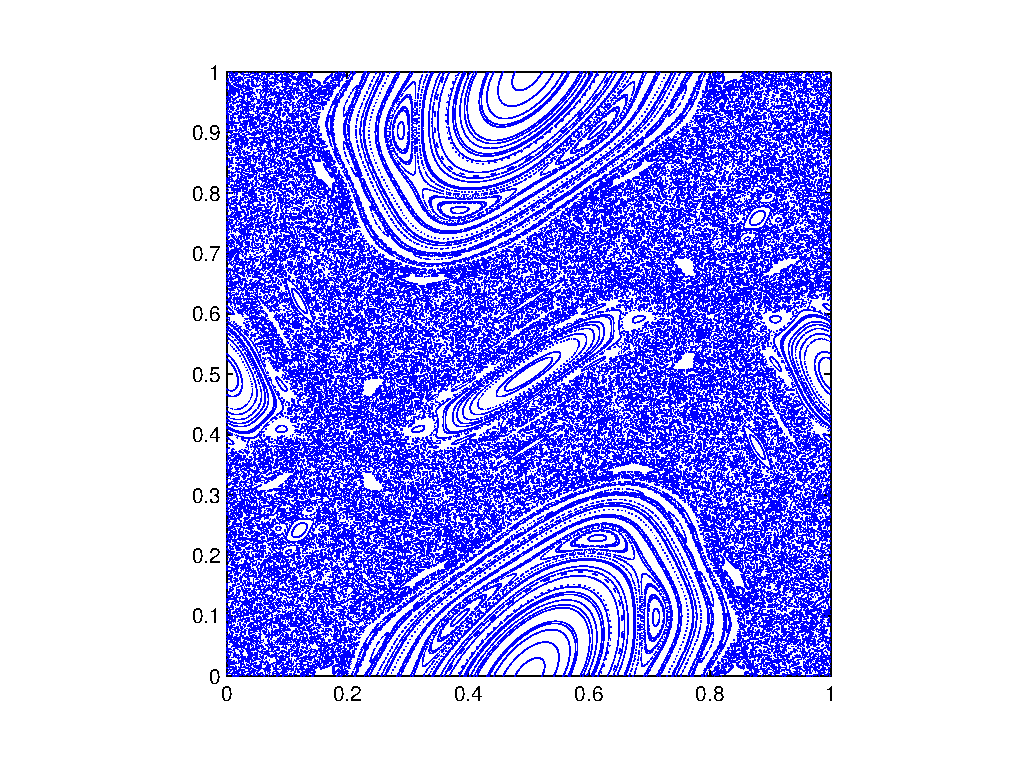
\includegraphics{standardmapdotplot.eps}}}
\end{figure}

%\begin{figure}
%\caption{\label{standardmapsimuexact} $\text{cos}(x)$ function
%evolved by standard map for 40 iterations}
%\centerline{\scalebox{0.5}[0.5]{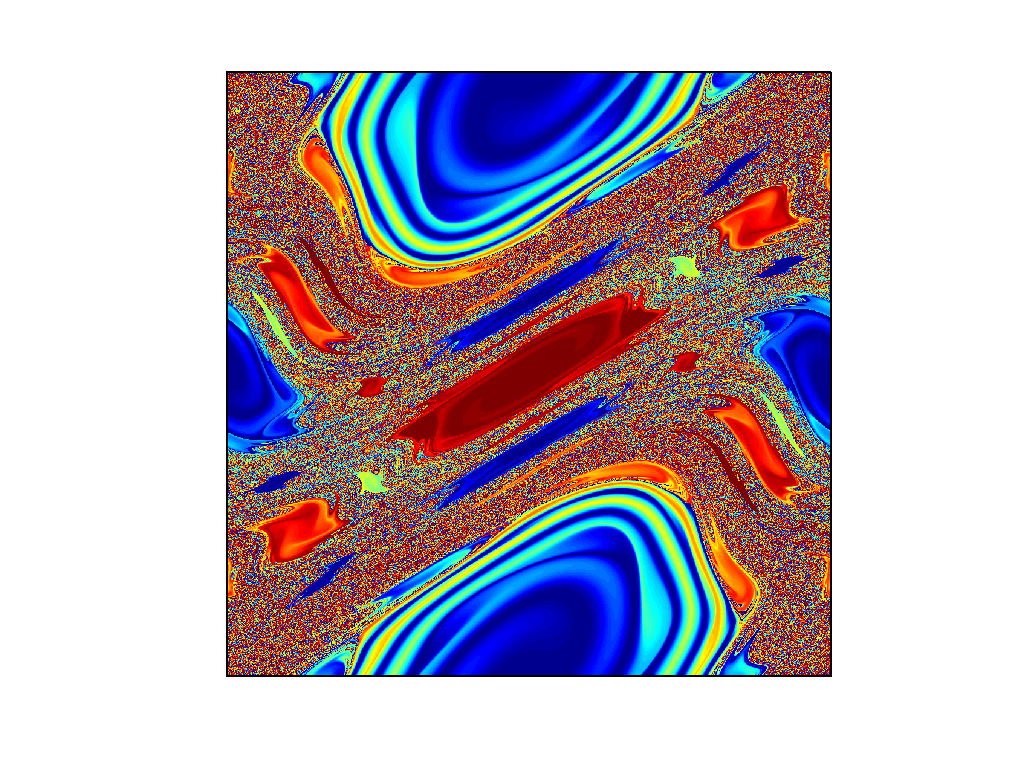
\includegraphics{standardmapsimuexact.eps}}}
%\end{figure}

%\begin{figure}
%\caption{\label{standardmapsimumarkov} $\text{cos}(x)$ function
%evolved by the Markov chain model of standard map for 40 iterations
%}
%\centerline{\scalebox{0.5}[0.5]{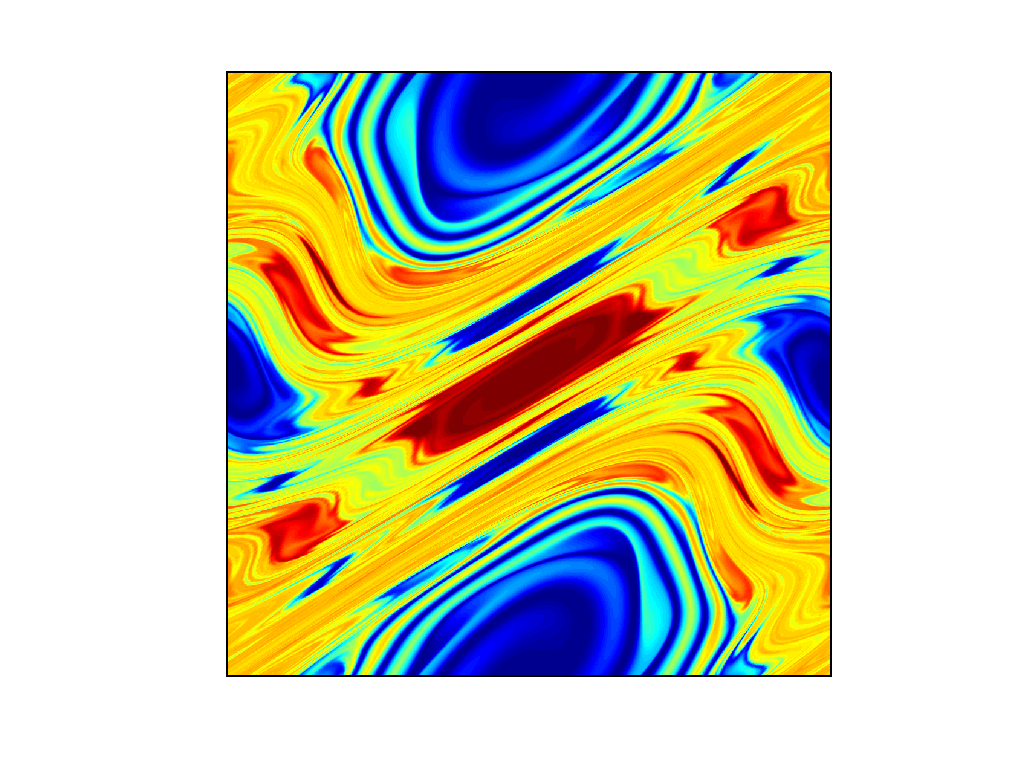
\includegraphics{standardmapsimumarkov.eps}}}
%\end{figure}


\begin{figure}
\centerline{
\scalebox{0.5}[0.5]{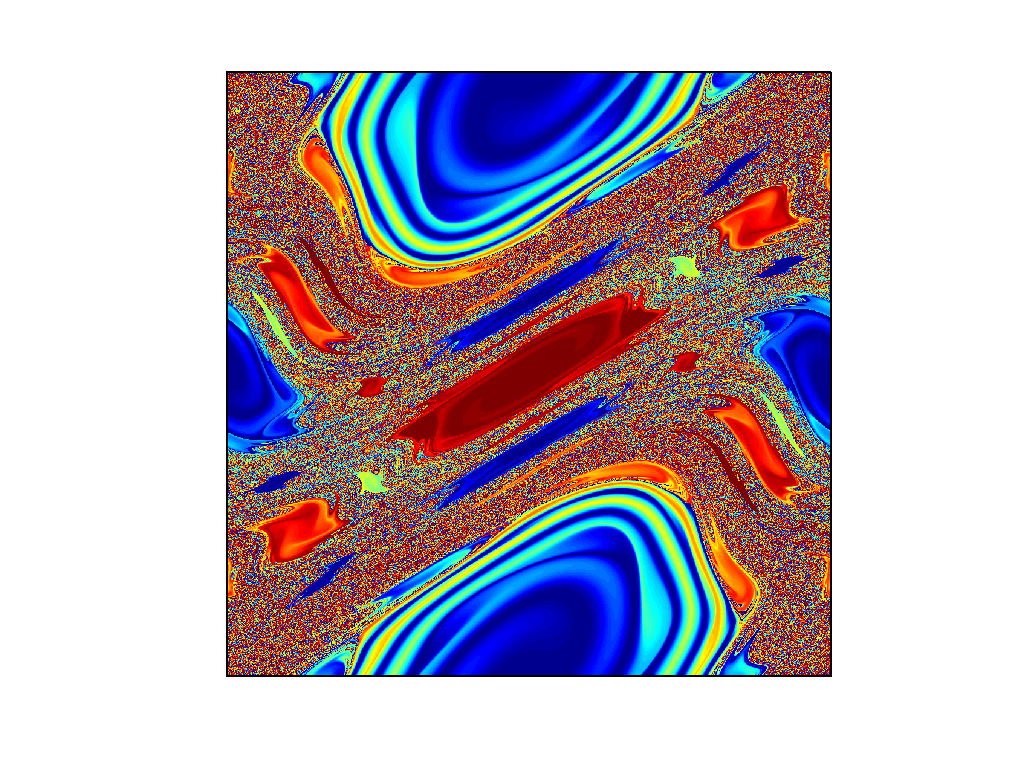
\includegraphics{standardmapsimuexact.eps}}
\scalebox{0.5}[0.5]{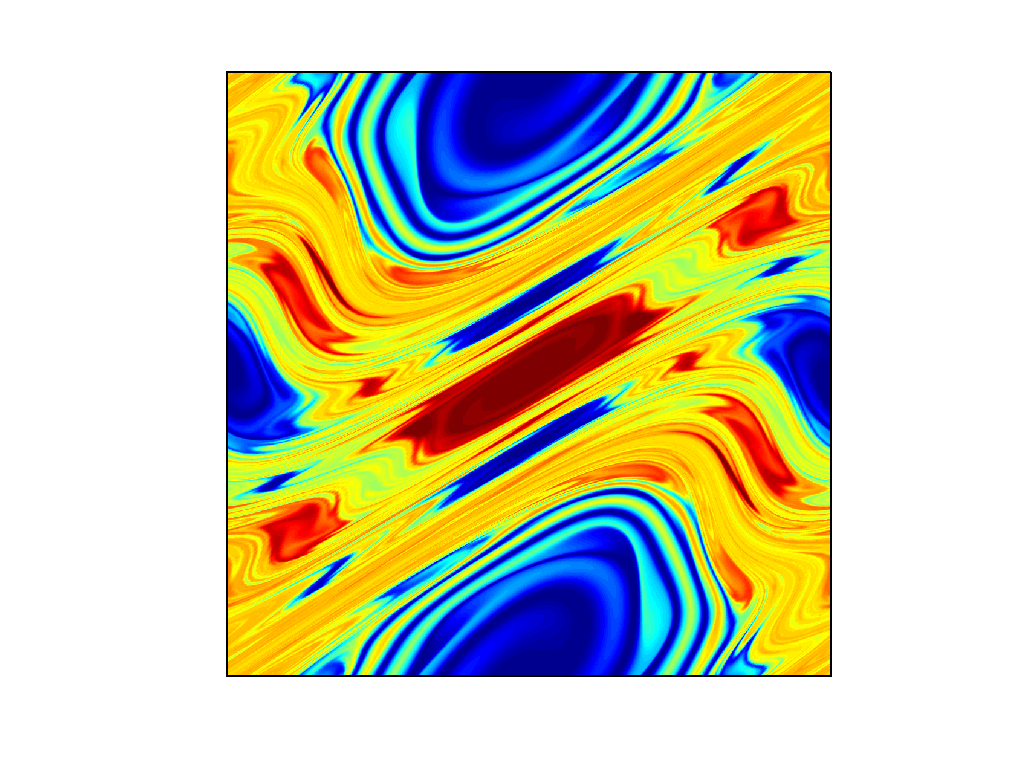
\includegraphics{standardmapsimumarkov.eps}} }
\caption{\label{standardmapsimuexact}  $\text{cos}(x)$ function
evolved by standard map for 40 iterations}
\caption{\label{standardmapsimumarkov} $\text{cos}(x)$ function
evolved by the Markov chain model of standard map for 40 iterations}
\end{figure}


The Markov model will serve as our main tool to study the effect
when more diffusion is added to the map. Thus before we do that, we
should first justify how large the diffusivity rate is for the
Markov model.

%%%%%%%%%%%%%%%%%%%%%%%%%%%%%%%%%%
\subsection{About the Error}
%%%%%%%%%%%%%%%%%%%%%%%%%%%%%%%%%%
In this subsection we derive the error of the $P_h$ operator after
one iteration. This algorithm is first order accuracy to approximate
the Perron-Frobenious operator.


Let $\mathbf{x}_i = (x_i,y_i)$ be the center of cell $a_i$, and $f_i
= f(\mathbf{x}_i)$ denotes the function value at $\mathbf{x}_i$, and
$F_i$ is the function value calculated by our algorithm. Let
$\mathcal{J}_i = \{j | S^{-1}(a_i) \cap a_i \neq \emptyset\}$. Now
suppose at iteraiton $l-1$ the function $f_j^{l-1}$ is known exactly
for every $j \in \mathcal{J}$. Define the error of $P_h$ on cell $i$
at iteration $l$ to be $e_i^l$,
\begin{eqnarray}
e_i^l = F_i^l - f_i^l
\end{eqnarray}
where $F_i^l$ can be represented by the $P_h$ operator and $f_j^{l-1}$,
\begin{eqnarray}
F_i^l = \sum_{j \in \mathcal{J}_i} (P_h)_{ij} f_j^{l-1}
\end{eqnarray}
and now we Taylor expand $f_j^{l-1}$ about $f(S^{-1}(\mathbf{x}_i))$,
\begin{eqnarray}
f_j^{l-1}  = f^{l-1}(\mathbf{x}_i) +
\frac{\partial{f^{l-1}}}{\partial{\mathbf{x}_i}}
(\mathbf{x}_j-S^{-1}(\mathbf{x}_i))
           + \text{O}((\mathbf{x}_j-S^{-1}(\mathbf{x}_i)^2))
\end{eqnarray}
Substitute above relations into the error equation, one has
\begin{eqnarray}
e_i^l = \sum_{j \in\mathcal{J}_i} (P_h)_{ij}
\left(f^{l-1}(S^{-1}(\mathbf{x}_i))
        + \frac{\partial{f^{l-1}}}{\partial{x}} (\mathbf{x}_j-S^{-1}(\mathbf{x}_i))
        + \text{O}((\mathbf{x}_j-S^{-1}(\mathbf{x}_i)^2))\right) - f_i^l
\end{eqnarray}
Note that in any of our simplifications,
\begin{eqnarray}
f_i^l = \sum_{j \in \mathcal{J}_i} (P_h)_{ij}
f^{l-1}(S^{-1}(\mathbf{x}_i))
\end{eqnarray}
because $P_h$ is a stochastic matrix. Therefore one concludes

\begin{eqnarray}
e_i^l = \sum_{j \in \mathcal{J}} (P_h)_{ij} \left(
\frac{\partial{f^{l-1}}}{\partial{\mathbf{x}}}
(\mathbf{x}_j-S^{-1}(\mathbf{x}_i))) + \text{O}((\mathbf{x}_j-S^{-1}(\mathbf{x}_i)^2))\right)
\end{eqnarray}
$(P_h)_{ij}$ is the weighted area ratio. Clearly no matter it is
calculated by (\ref{arearaitioeq}) and then normalized or by (\ref{P
definition}) numerically, the error does not scale with $h$. The
$(\mathbf{x}_j-S^{-1}(\mathbf{x}_i))),{j \in \mathcal{J}_i}$ term is
the $x$ and $y$ distance of $S^{-1}(\mathbf{x}_i)$ to the grid
points, so it scales with $h$. Thus we can conclude this algorithm
has first order accuracy and when $h \rightarrow 0$, $F_i^l$
converges to $f_i^l$.

% scales with ???

One can view the above error $e_i^l$ as some artificial diffusion on
grid $i$. Because of this artificial diffusion, the operator $P_h$
is in fact more close to $[P(D^*,1)]$ rather than $[P]$. Although
$e_i^l$ is not uniform over the domain and scales different from the
physical diffusion $D^*$, we can still find an equivalent $D^*$ for
every $P_h$, and when


%%%%%%%%%%%%%%%%%%%%%%%%%%%%%%%%%%
\subsection{Estimation of $D^*$}
%%%%%%%%%%%%%%%%%%%%%%%%%%%%%%%%%%
As we have stated above, the operator $P_h$ is an approximation of
$[P(D^*,1)]$. Now let us assume one can equate the following
\begin{eqnarray}
\label{PnandP}
 P_h[d_h] = [d_h][M(D^*,1)][P]
\end{eqnarray}
and the diffusion caused by $[d_h]$ is small enough comparing with
$D^*$. we now discuss how to estimate $D^*$ when a $P_h$ is given.
Moreover, we also show that $D^*$ is roughly independent of what
function $P_h$ operates on.


To do this, we can create a test function $\phi(\mathbf{x})$ such
that $[P]\phi(\mathbf{x})$ is known analytically, and then apply it
to the the both sides of (\ref{PnandP}). We get
\begin{eqnarray}
\label{PnandPphi}
 P_h[d_h]\phi(\mathbf{x}) = [d_h][M(D^*,1)][P]\phi(\mathbf{x})
\end{eqnarray}
Left hand side of (\ref{PnandPphi}) can be evaluated numerically and
right hand side of it is done analytically and written as a function
of $D^*$. Thus we can solve for $D^*_\phi$ for this specific
$\phi(\mathbf{x})$.

The set of test functions we choose are $\phi_{k_1,k_2}$ for
$k_1,k_2\in \mathbb{Z}^+$ such that $\phi_{k_1,k_2}(\mathbf{x}) =
\sin(2\pi k_1 x^s)\sin(2 \pi k_2 y^s)$, where $[x^s , y^s]=S(x,y)$.
This particular choice satisfies $[P]\phi_{k_1,k_2}(\mathbf{x})=
\phi_{k_1,k_2}(S^{-1}(\mathbf{x})) = \sin(2\pi k_1 x)\sin(2 \pi k_2
y)$ and thus
\begin{eqnarray}
\label{MPphi}
 [M(D^*,1)][P]\phi_{k_1,k_2}(\mathbf{x}) = \sin(2\pi k_1 x)\sin(2 \pi k_2
y)\text{e}^{-4 \pi^2 (k_1^2+k_2^2)D^*}
\end{eqnarray}
Substitute the above equation to (\ref{PnandPphi}) and calculate the
2-norm of both sides, one can easily get the average of
$D^*_{\phi_{k_1,k_2}}$ over the domain $T^2$. The result of
estimated $D^*_{\phi_{k_1,k_2}}$ for $k_1=k_2 = k$ is plotted in
figure \ref{estimateddiffusionrate}.

Because in the process of approximating the map by a Markov matrix,
the diffusion is not added uniformly, one should not get a perfectly
consistent $D^*$ for every function and for the whole domain.
However, in figure \ref{estimateddiffusionrate} one can clearly see
when $n$ is large enough, $D^*_{\phi_{k_1,k_2}}$ is close to a
constant for different wave numbers $k$. The reason that all the
curves drop when $k$ gets higher is because the $[d_h]$ operator
itself is diffusive and this effect is not ignorable when $k$ is
large. One should not expect $n=50$ to capture any correct
information with wave number higher than $25$!

This figure gives us the idea of how large the augmentative
diffusivity rate is when $P_h$ is used to replaced $[P]$ and only a
range of wave number is considered.

We choose $D^* = D^*_{\phi_{1/10h,1/10h}}$ as the nominal diffusion
rate for $P_h$. It is not surprising that $D^*_{\phi_{1/10h,1/10h}}$
is linear to $\frac{1}{1/h^2}$. In figure \ref{ndchart} $P_h$ of
several different maps are calculated, and the
$D^*_{\phi_{1/10h,1/10h}}$ is then estimated by the above method.
Clearly one has
\begin{eqnarray}
\label{MPphi} D^*_{\phi_{1/10h,1/10h}} = c_s h^2
\end{eqnarray}
for some constant $c_s$, which is different from map to map.




%\begin{figure}
%\caption{\label{estimateddiffusionrate} The estimation of $D^*$ for
%different number of grids, as a function of wave number}
%\centerline{\scalebox{0.5}[0.5]{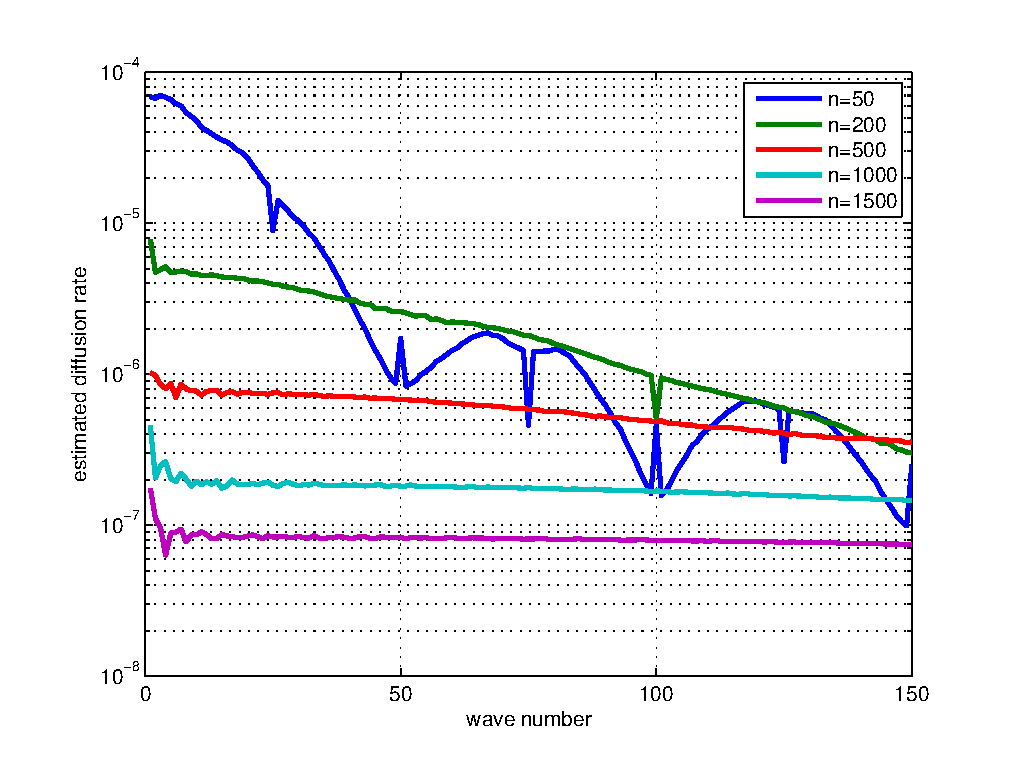
\includegraphics{estimateddiffusionrate.eps}}}
%\end{figure}
%\begin{figure}
%\caption{\label{ndchart} $D^*$ as a function of $\frac{1}{n^2}$, for
%different maps }
%\centerline{\scalebox{0.5}[0.5]{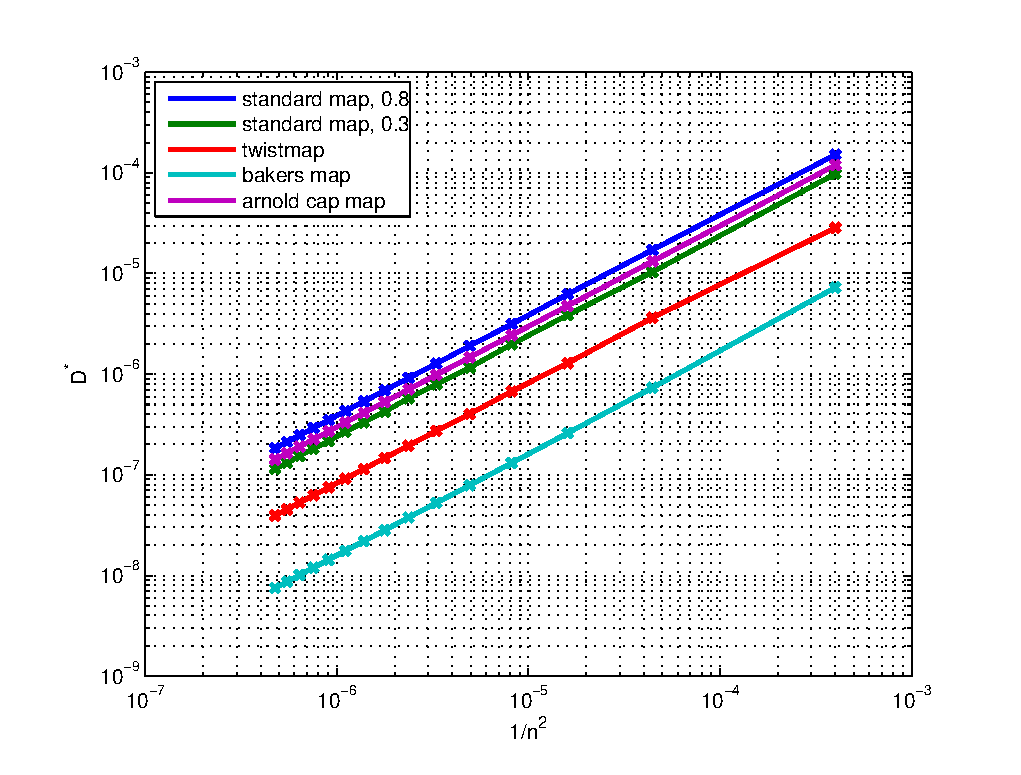
\includegraphics{ndchart.eps}}}
%\end{figure}


\begin{figure}
\centerline{\scalebox{0.5}[0.5]{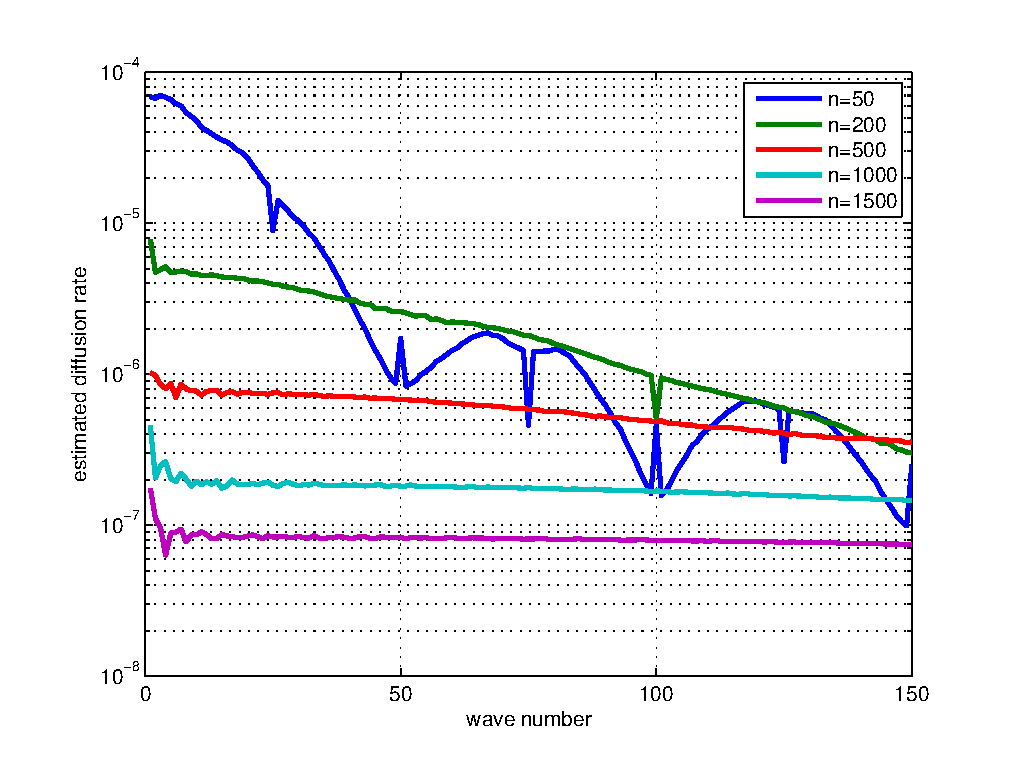
\includegraphics{estimateddiffusionrate.eps}}
            \scalebox{0.5}[0.5]{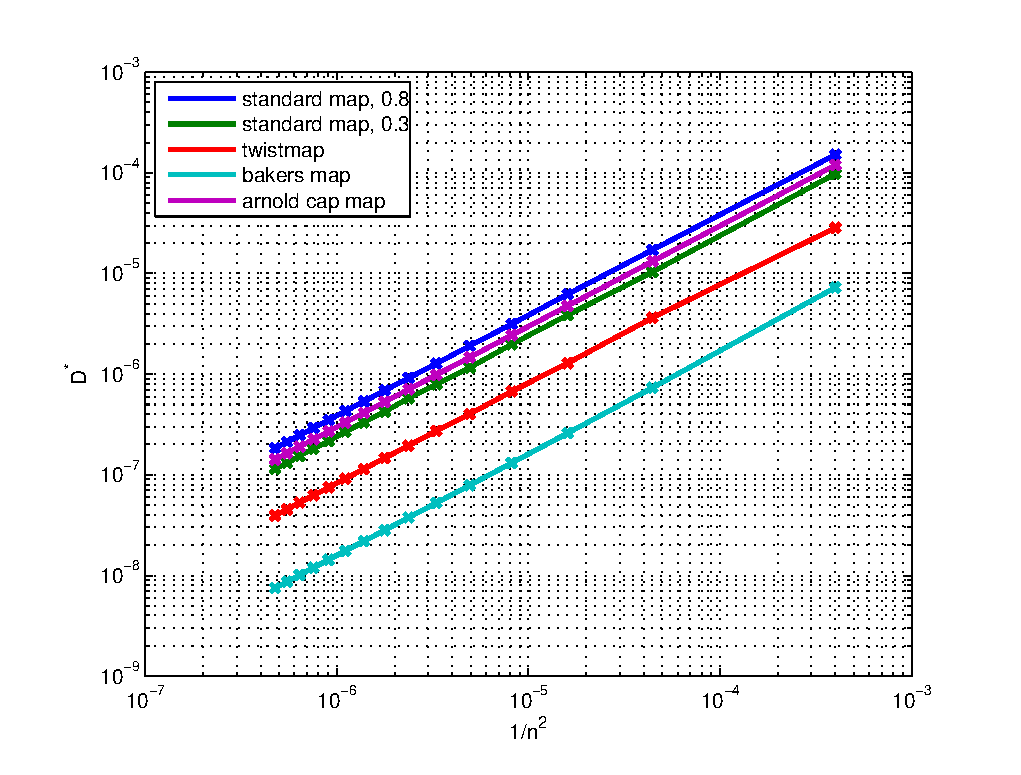
\includegraphics{ndchart.eps}}}
\caption{\label{ndchart} $D^*$ as a function of $h^2$, for
different maps } \caption{\label{estimateddiffusionrate} The
estimation of $D^*$ for different number of grids, as a function of
wave number}
\end{figure}

\subsection{Optimization of Mixing Protocol}
The goal of this $P_h$ operator is to deal with the design problem of microfluidic channels.
More speficifically, we formulate a periodical microfluidic channel as a map-with-diffusion
operator, and thus it can be optimized when certain objective function is given. The detail
of the formulation will be discussed later. Here we would like to address the scale issues.

As we have disscussed in the previous section, the diffusivity rate $D^*$ of $P_h$ is
proportional to $h^2$. Practically, one can add more diffusion without any difficulty,
but the only way to reduce the diffusion is to use a larger $1/h$. Here we would like to give a
rough estimation of the number on $1/h$ one needs when physical parameters are considered.

We adopt the parameters used in \ref{stroock2002}. Consider mixing a stream of protein
solution in aqueous buffer: molecular weight $10^5$, molecular diffucivity
$D_m~10^{-6} \text{cm}^2/\text{s}$. The mixing channel has cross sectional dimension
$200\mu \text{m}$ and length around $3\text{cm}$. Converting this set of parameters to a unit
square where $P_h$ operater is calculated from, one can deduce the diffucivity rate needed is
around $D =5 \times 10^{-5}$. According to figure \ref{estimateddiffusionrate}, $1/h=500$ is quite
sufficient for every map.







%%%%%%%%%%%%%%%%%%%%%%%%%%%%%%%%%%
\section{A Frequency Domain Approach}
\label{A Frequency Domain Approach}
%%%%%%%%%%%%%%%%%%%%%%%%%%%%%%%%%%

We would like to also discuss a model of the map with diffusion in
frequency domain. The goal of this model is not to simulate the map
with diffusion in a simpler way or to provide us an objective
function to optimize. Instead, we use the frequency domain model to
study how diffusion enhances the mixing.


\subsection{The Model and the Simplifications}

 We Fourier expand $w_n$ in
2-d,
\begin{eqnarray}
(w_h)_{p,q} =\sum_{s=0}^{1/h-1} \sum_{r=0}^{1/h-1} (\hat{w}_h)_{r,s}
e^{2 \pi j p rh} e^{2 \pi j q sh}  \mbox{   for }p,q \in
\{0,1,...,1/h-1\}
\end{eqnarray}
where $j = \sqrt{-1}$. The inverse discrete Fourier transform is
linear so we can rewrite the above equation as,
\begin{eqnarray}
w_h = F^{-1} \hat{w}_h
\end{eqnarray}
where $F^{-1} \in \mathbb{C}^{1/h^2 \times 1/h^2}$, $F^{-1}_{rs,pq}
=e^{2 \pi j h ({pr}+{qs}) i}$ for $p,q,r,s = 0,...,1/h-1$. Similarly the
forward transform can be denoted as $F$. Substitute the transforms
into the relation $w_h^{l+1} = P_h w_h^l$, one gets
\begin{eqnarray}
\hat{w}_h^{l+1} &=&F P_h F^{-1} \hat{w}_h^l \nonumber\\
          &\equiv& \hat{P}_h \hat{w}_h^l
\end{eqnarray}
Even though we have a really sparse $P_h$, the two dense matrices
$F$ and $F^{-1}$ spoil all the sparsity. Hence it is not wise to
evolve the system in frequency domain. However, just like in the
space domain, most of the entries in $\hat{P}_h$ could be very small.
Making those small entries zero, one can perhaps result in a sparse
operator in the frequency domain again. Nonetheless, the computation
cost is already huge when deciding which entry can be ignored, and
the operator one gets is far less sparser than $P_h$ in general.

Therefore, a further simplification is required to make the problem
more achievable. Let us start from observing what the most important
components are in frequency domain when a system evolves. Selecting
these components out of the others is our basic strategy to reduce
the size of of the model.


Suppose we only focus on a certain set of initial conditions, for
example, if one chooses $w_h^0 = [d_h][\cos(x)]$, then $\hat{w}_h^0$
has only a single nonzero component. As the system evolves,
$\hat{w}_h^l$ gets more and more non-zeros. Meanwhile, each of the
components also decays in various rates. And finally, when the two
effects balance, the system arrives at its eigenfunction direction,
which only has a limited number of nonzero frequencies. In this
whole procedure, three simplifications can be done:
\begin{itemize}
  \item We restrict the initial condition to be some simple
  functions, which do not have too many components in the frequency
  domain.
  \item When the system evolves, we keep recording the states it
  passes through. We set a threshold, and only the states whose
  absolute values are higher than the threshold are kept. Thus we can get how
  many significant $m$ states we needs to simulate the system.
  \item The reduced operator, called $\hat{P}_m \in \mathbb{C}^{m \times m}$,
  is formed by selecting the corresponding entries in $\hat{P}$. When
  doing this, we also set the entries whose absolute values are
  below the threshold to be zero.
\end{itemize}

It seems very restrictive when we say the initial condition is a
"simple function". Nonetheless, considering that we are studying the
mixing property of a map, to begin with a simple function which has
only few nonzeros in frequency domain is actually reasonable.
Moreover, on the 2-d domain with $1/h$ by $1/h$ grids, even for a step
function in $x$-direction has only $1/h$ nonzero components-still
pretty sparse.

The second simplification is the key to decide the size of the
reduced system. One can certainly image how the number of nonzero
states grows when the system evolves-it grows exponentially.
However, most of the components are mapped from low frequency states
to high frequency ones. This means a large amount of them decays
fast and becomes insignificant before the system arrived at its
stationary state. Deleting these states from our simulation should
not affect too much. Besides, one can always adjust the threshold
value to move between a more accurate model and a compact one.

The above step is equivalent to
\begin{eqnarray}
\label{Prmodel}
    \hat{P}_m(D^*) = F_m P_n(D^*) F_m^T
\end{eqnarray}
where $F_m$ is composed by the selected rows of $F$, and because $F$ is unitary, $F^{-1} = F^T$,
$F_m^T$ is the selected columns of $F^{-1}$. If the number of selected states is much smaller than
$1/h^2$, the $\hat{P}_m$ model can be evolved efficiently.

Suppose the selected $m$ states have indice $(r_i,s_i)$, for $i=1,...,m$
in the 2-d representation of $\hat{w}_h$, and each of them has the
corresponding wave number $\mathbf{k}_i = \sqrt{(k_1)_{r_i}^2+(k_2)_{s_i}^2}$.
Let $\hat{k}_m = [\mathbf{k}_1, \mathbf{k}_2,...,\mathbf{k}_m ]$.
If one want to study how the system behavior changes when more diffusion is added.
It is equivalent to pre- or post-multiply the $\hat{P}_r$ model by a diagonal matrix,
\begin{eqnarray}
\label{PraddDiffusion}
    \hat{P}_m(D) = \hat{P}_m(D^*)\text{e}^{-4 \pi^2 (D-D^*) \text{diag}(\hat{k}_m^2)}
\end{eqnarray}

If the above simplifications have resulted in a moderate size system,
the thrid part is not necessary. However, setting the small nonzeros
zero helps us to identify the most important paths which connect the
initial condition to the stationary state.



\subsection{Simulations}
We set the threshold value in the second and the third steps of simplifications
 to be $0.01$. In figure \ref{PrchangeD} we compare the $P_h$ model and the $\hat{P}_m$ model for
standard map with $\epsilon=0.2$ and initial condition $\cos(x)$. In the $P_h$ model, we use fixed number of grid $1/h = 200$.
The corresponding $D^*$ is $4.21e-6$ and number of states is $1/h^2 = 40000$. The solid lines show the $P_h$ model with some augment diffusion added by using
Discrete Fourier transform technique on $w_h^l$ after every iteration. $\hat{P}_m$ model is calculated by
equation (\ref{Prmodel}) using the raw $P_h(D^*)$ model. The $\hat{P}_m$ model has only $4326$ states. Its diffusion is added by applying equation (\ref{PraddDiffusion}) and plotted in dased lines.

The main advantage of the $\hat{P}_m$ model is of course not in the simulation. It provides us an efficient way to study how the diffusion affects the system behavior. Suppose we focus on the exponentional region of the convergence curve, figure (\ref{Dvslambda}) shows how the diffusion affects the decay rate when the system is in its eigenvector direction. The map is standard map with various chaotic parameters $\epsilon$. Although the theorem about the eigenvalue perturbation when a diagonal matrix is multiplied is not known. The numerical simulations do show a roughly linear relation when $\epsilon$ is small.




\begin{figure}
 \centerline{
  \scalebox{0.5}[0.5]{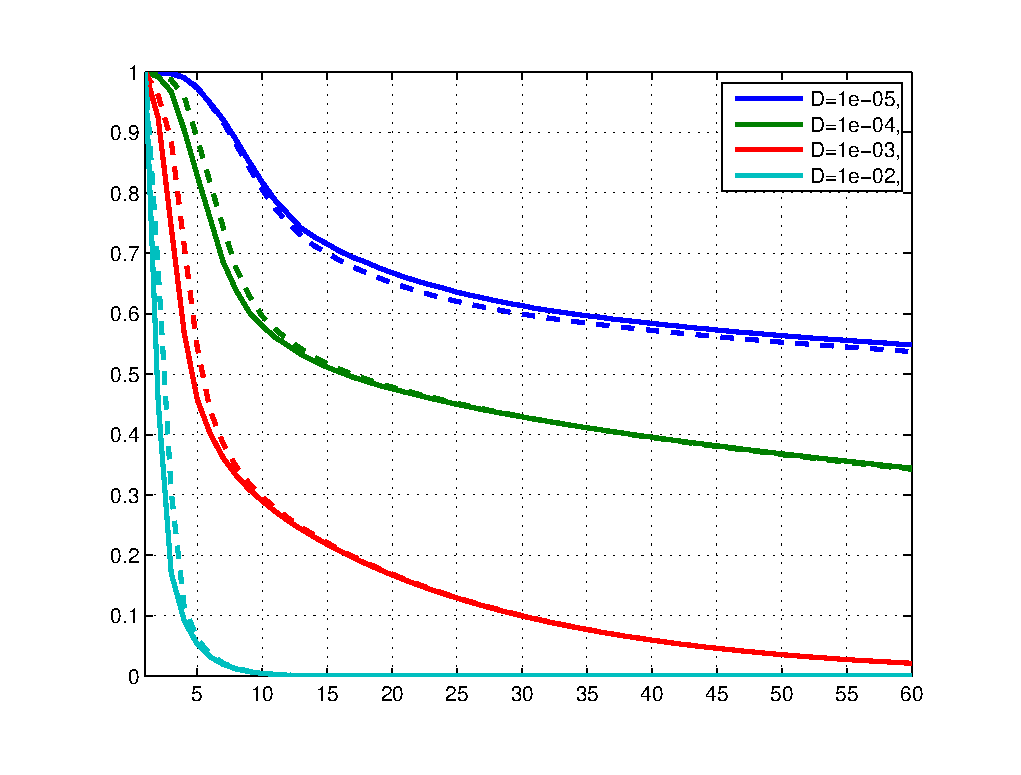
\includegraphics{PrchangeD.eps}}
  \scalebox{0.5}[0.5]{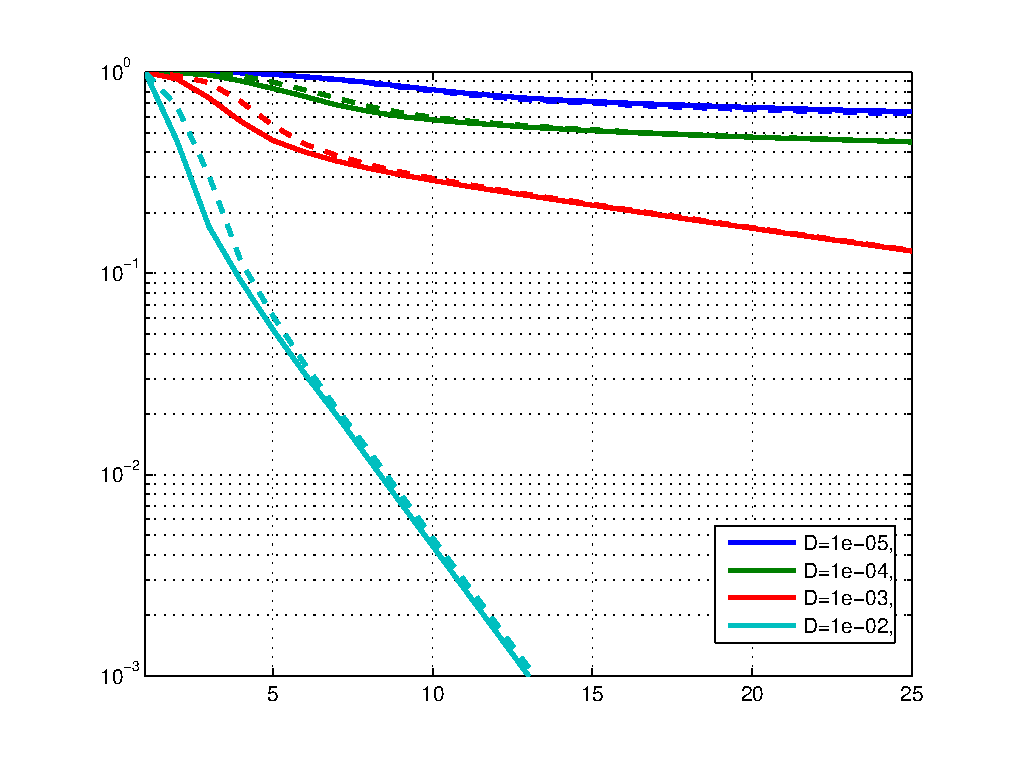
\includegraphics{PrchangeDlog.eps}}
} \caption{ddd}
  \label{PrchangeD}
\end{figure}


\begin{figure}
 \centerline{
  \scalebox{0.5}[0.5]{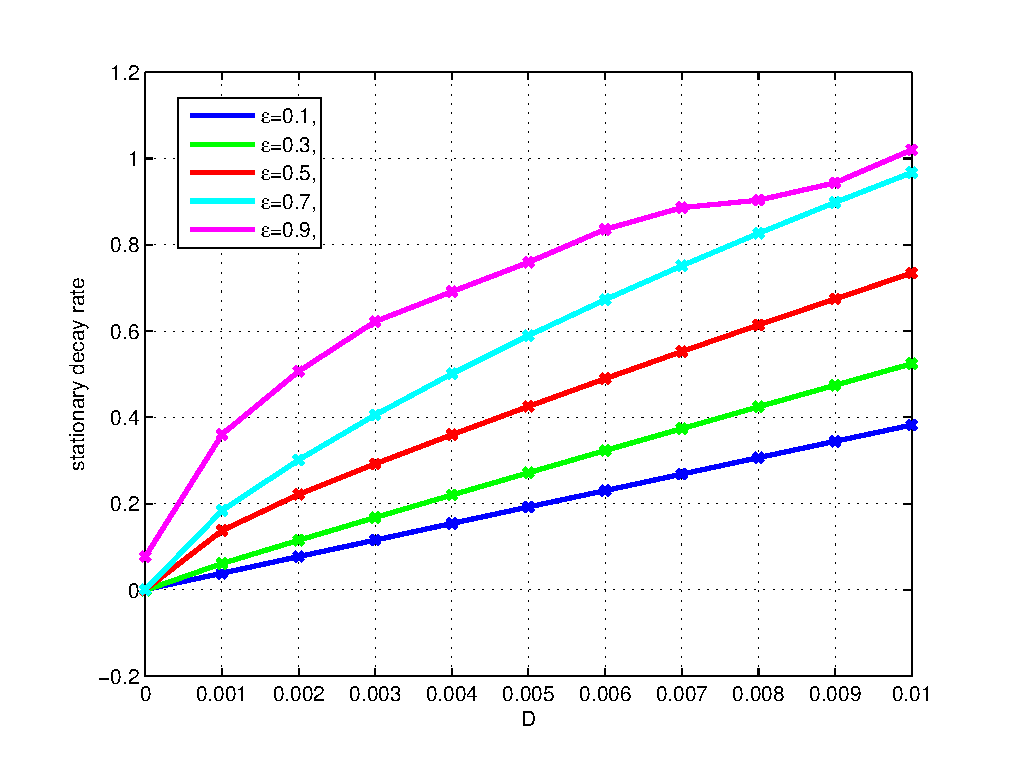
\includegraphics{Dvslambda.eps}}
} \caption{ddd}
  \label{Dvslambda}
\end{figure}


\subsection{Mixing Enhancement Factor}

%%%%%%%%%%%%%%%%%%%%%%%%%%%%%%%%%%
\section{Thoughts of Cut-off Phenomenon}
\label{Thoughts of Cut-off Phenomenon}
%%%%%%%%%%%%%%%%%%%%%%%%%%%%%%%%%%
In many Markov chian simulations, one can observe a 2 or 3-stage
convergence rate change just like we see in the nonlinear
map-with-diffusion simulations. For linear systems like Markov
chains, analyzing of the eigen-structure and the non-normal feature
of the Markov matrices gives us the idea of how the cut-off happens.
Nonetheless, it shows less physical reason of why a system has
cut-off. On the other hand, people has studied this multi-stage
chage and linked it to the physical mixing property of a
map-with-diffusion operator in the nonlinear map researches. We
think these two fields are tightly related. More percisely, the
cut-off phenomenon in a linear system is actually an imitation of
the nonlinear behavior of some (probably simpler) systems.


We first state the definition of the cut-off given by Diaconis in
\ref{Diaconis2005} Assume that, to any finite set $\Omega$ and any
pair of probability measures $\mu$, $\nu$ on $\Omega$ is associated
a real number $D(\mu,\nu)$ such that $D(\mu,\nu)\in [0,1]$

\begin{eqnarray}
\max_{\Omega,\mu,\nu} D(\mu,\nu) = 1
\end{eqnarray}
and $D(\mu,\nu)=0$ if and only if $\mu=\nu$. Consider a sequence of
(finite) probability spaces $(\Omega_n,\nu_n)$, $n=1,2,...$, each
equipped with a sequence of probability measure $\mu^k_n$,
$l=0,1,...$, such that
\begin{eqnarray}
\lim_{k \rightarrow \infty} D(\mu^k_n,\nu_n)=0
\end{eqnarray}
The definition of a cut-off is,

\begin{definition}
\label{cutoffdefition}
(Diaconis) A family $(\Omega_n,\nu_n, (\mu^k_n)_{k=0,1,...})_{n=1,2,...}$
presents a D-cut-off if there exists a sequence $(t_n)$ of positive
reals such that, for any $\epsilon \in(0,1)$,
\begin{enumerate}
  \item $\lim_{k \rightarrow \infty}D(\mu^k_n,\nu_n) = 0 \mbox{ if }
  k_n>(1+\epsilon)t_n$
  \item $\lim_{k \rightarrow \infty}D(\mu^k_n,\nu_n) = 1 \mbox{ if }
  k_n<(1+\epsilon)t_n $
\end{enumerate}
\end{definition}

One example of a family of $\varphi^k_n \equiv D(\mu_k^n,\nu_n)$ sequence
is shown in figure \ref{democutoff1} (a). Define the D-mixing time
\begin{eqnarray}
\label{Dmixingtime}
\tau^D_n=\tau^D_n(\epsilon) = \inf\{k\,:\,D(\mu_k^n,\nu_n) \le \epsilon\}
\end{eqnarray}
If we normalize the trajectories in figure \ref{democutoff1} (a) by their $\tau_n^D(0.5)$, the
normalized trajectories are shown in figure \ref{democutoff1} (b).
Definition \ref{cutoffdefition} restrice the maximum of diatance D to 1.
However, this can be easily extended to the case where D is unbounded \ref{Diaconis2005},
e.g., the $L^2$ distance
\begin{eqnarray}
\label{L2distance}
 D(\mu,\nu) = \left(  \sum_{\omega \in \Omega} | \frac{\mu(\omega)}{\nu(\omega)}-1 |^2 \nu(\omega) \right)^{1/2}
\end{eqnarray}
In this case, the limit value $1$ in definition \ref{cutoffdefition} should be replaced by $\infty$.
An example of this kind of cut-off trajectories and the normalized one are shown in figure \ref{democutoff2} (a)(b). \ref{} discusses the
$L^2$ cut-off phenomenon in detail. Other distance which are interesting are total variation distance, separation, etc. Please refer to \ref{Diaconis2005} \ref{} for detail.
In this article, we will focus on the distance defined as
\begin{eqnarray}
\label{normalizedL2distance}
  D(\mu,\nu) = \frac{1}{|\Omega|^2}\left(  \sum_{\omega \in \Omega} | f(\omega)-1 |^2 \nu(\omega) \right)^{1/2}
\end{eqnarray}
where $f(\omega) = \frac{\mu(\omega)}{\nu(\omega)}$ and $|\Omega|$
is the cardinality of $\Omega$. This distance is unbounded but it
does not scale with $|\Omega|$. The reason we choose this measure is
it fits the measure we discussed in section \ref{Measure for Mixing}
better.


\begin{figure}
 \centerline{
  \scalebox{0.5}[0.5]{\includegraphics{democutoff1.eps}}
  \scalebox{0.5}[0.5]{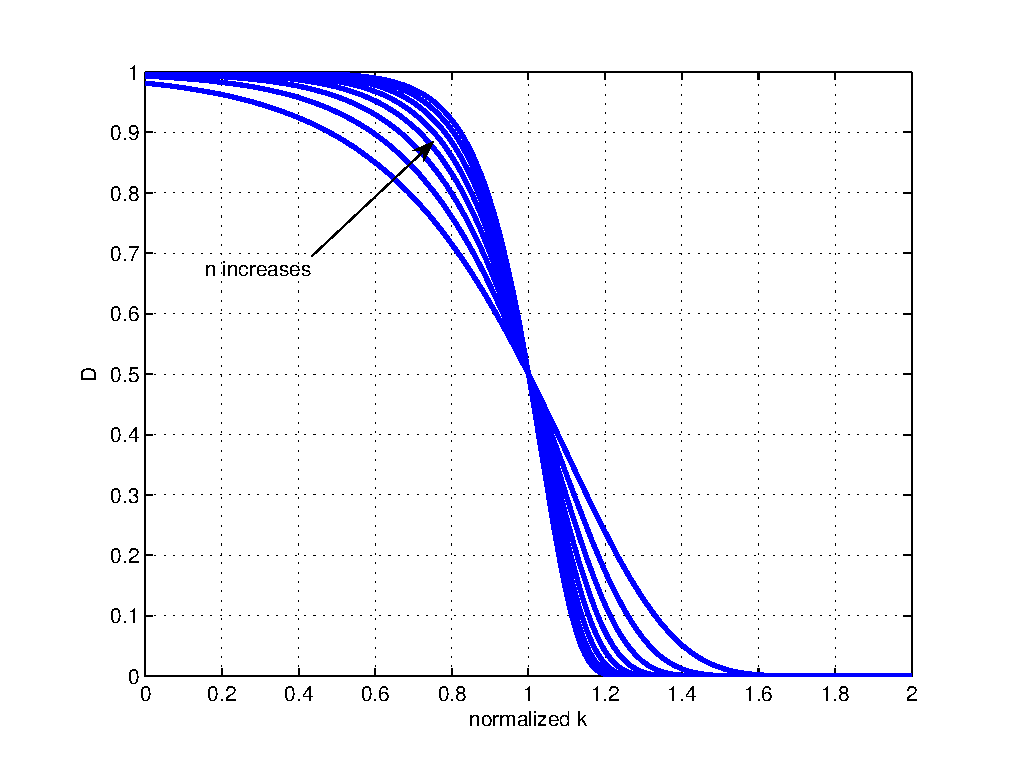
\includegraphics{democutoff1n.eps}}
} \caption{(a) A family of trajectories which present a cutoff, (b) the normalization of (a)}
  \label{democutoff1}
\end{figure}

\begin{figure}
 \centerline{
  \scalebox{0.5}[0.5]{\includegraphics{democutoff2.eps}}
  \scalebox{0.5}[0.5]{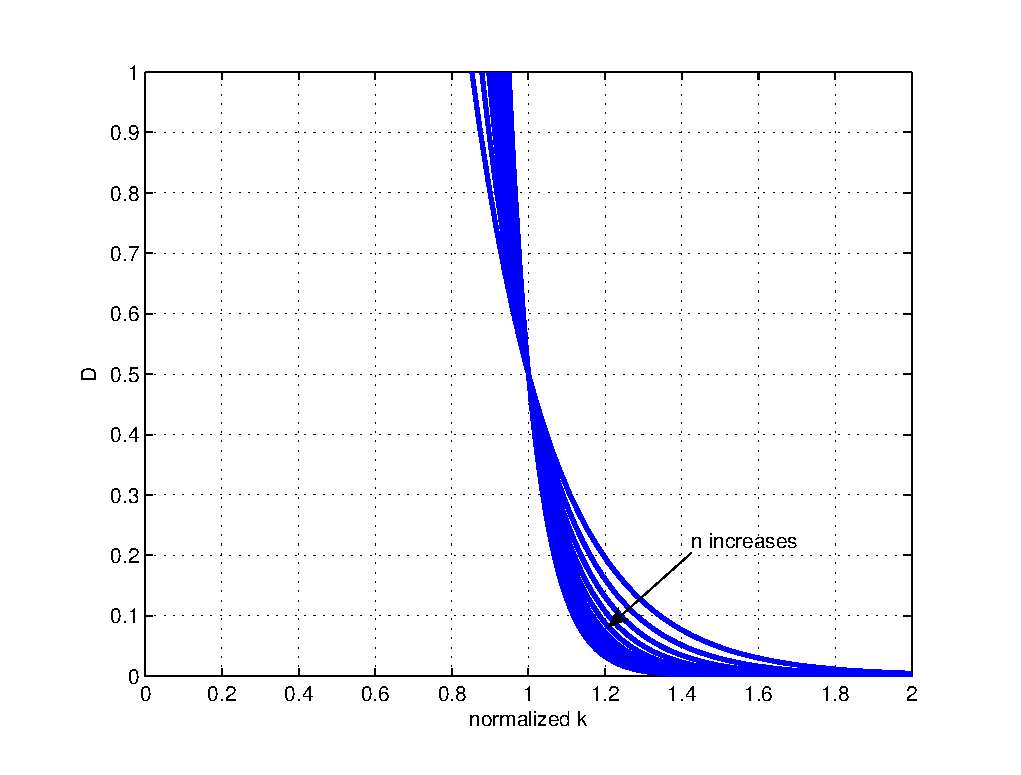
\includegraphics{democutoff2n.eps}}
} \caption{(a) A family of trajectories which present a cutoff when $D$ is unbounded above, (b) the normalization of (a)}
  \label{democutoff2}
\end{figure}






It is noticed that for some of the Markov chains which have
cut-offs, the rate of convergence before the exponentional decay
region is doubly exponentional. So let us begin with a function
which decays doubly exponentinally. Consider the following sequence,
 \begin{eqnarray}
 \label{doublyconvergence}
 \varphi^k_n = \text{e}^{-a^{k-n}}
 \end{eqnarray}
 where $a>0$ is a real number. It is easy to see that if $D(\mu^k_n,\nu_n)=\varphi^k_n
 $, the family $(\Omega_n,\nu_n, (\mu^k_n)_{k=0,1,...})_{n=1,2,...}$ satisfies the definition of cut-off. If
 one ask the question: what kind of linear system family has the above
 congergence property? The answer is not obvious at all. However one
 can easily find a family of nonlinear map-with-diffusion operator with varying diffucivity rate which possesses this
 convergence feature. Consider the following examples.

\begin{example}

Consider the baker's map on $T^2$,
  \begin{eqnarray}
    S(x,y) =  \left\{ \begin{array}{cc}
                 (2x,\frac{1}{2}y) \mbox{ mod } 1      &\mbox{, if } 0\le x < \frac{1}{2} \\
                 (2x,\frac{1}{2}(y+1)) \mbox{ mod } 1  &\mbox{, if } \frac{1}{2}\le x< 1\\
              \end{array} \right.
  \end{eqnarray}
with initial condition $c^0(\mathbf{x})= \pi^{\frac{1}{2}}\cos(2 \pi
y)$, diffusion operator with diffucivity $D$ is applied after every
iteration. The problem is analytical solvable, and we have,
  \begin{eqnarray}
   c^l(\mathbf{x}) = \pi^{\frac{1}{2}}\text{e}^{-4 \pi^2 D 2 ^{2 l}}\cos(2 \pi 2^l
   y) \mbox{ for }l = 1,2,...
  \end{eqnarray}
and the 2-norm of $c^l(\mathbf{x})$ is
  \begin{eqnarray}
  \label{bakersmapconvergence}
   ||c^l(\mathbf{x})||_2 = \text{e}^{-4 \pi^2 D 2 ^{2 l}}
  \end{eqnarray}
Comparing (\ref{bakersmapconvergence}) with
(\ref{doublyconvergence}), if let $l=k$, $a=4$ and $D =\frac{4^{-n-1}}{\pi^2}$,
one can certainly build the convergence sequence.
\end{example}

In fact a simple linear map can achieve this goal
\begin{example}

Consider Arnold's cat map on $T^2$,
  \begin{eqnarray}
               x' \leftarrow  2x+y (\mbox{ mod } 1)\\
               y' \leftarrow  x+y (\mbox{ mod } 1) \nonumber
  \end{eqnarray}
with initial condition and diffusion the same as the previous
example. The map maps wave number in $x$ and $y$ directions as
  \begin{eqnarray}
  \label{wavenumberexp}
    \left[\begin{array}{c}
           k_1'\\
           k_2'
    \end{array}\right] =
    \left[\begin{array}{cc}
           1& -1\\
           -1& 2
    \end{array}\right]
    \left[\begin{array}{c}
           k_1\\
           k_2
    \end{array}\right]
               %k_1' &=& k_1  - k_2 \\
               %k_2' &=& -k_1 + 2 k_2  \nonumber
  \end{eqnarray}
One can easily check that the magnitude of the wave number $(k_1,k_2)$
in (\ref{wavenumberexp}) grows exponentionally. Hence similiar to the Baker's
map example, the doubly exponentioal decay sequence can be easily built.
\end{example}

The above two examples show that we can create a family of
map-with-diffusion operator with indices $n$ which presents a
cut-off. If we apply the modeling procedures disscussed in section
\ref{The Markov Chain Model of a Map} and \ref{A Frequency Domain
Approach} to the above examples, and the grid size $h$ is small
enough to capture the doubly exponential convergence corrcectly up
to $\tau^D_n$ , we can surly get the corresponding finit dimensional
linear map which presents a cutoff. Because it is just a finite
dimensional linear model, finally the state has to evolve to one of
its eigenvector direction. 


%%%%%%%%%%%%%%%%%%%%%%%%%%%%%%
\subsection{Cutoff and Mixing}
\label{Cutoff and Mixing}
%%%%%%%%%%%%%%%%%%%%%%%%%%%%%%
A cutoff means the distance to stationary stays high for a while and then drops
to it rapidly. If we use the this kind of map as a mixing protocol, an optimal
number of iterations can be certainly found.

However, in the above two examples, the magnitude of wave number grows exponentially
with fairly large rates. One may doubt whether this happens in a real mixing protocol.
The following example shows the possibility.

\begin{example}
\label{LTM example}
We consider a simplified Linked Twist Map (LTM) defined in \ref{Wiggins2004}. This map
is composed by two twist map with radius $0.3$ and center at $(0.4,0.4)$ and $(0.6,0.6)$,
respectively. The LTM is defined by applying the two twist map 10 times each, i.e,
\begin{eqnarray}
 P^{LTM}_{h} = (P_{h}^{TM_1}(D^*))^{10}(P_{h}^{TM_2}(D^*))^{10}
\end{eqnarray}
where $P_{h}^{TM_1}(D^*)$ and $P_{h}^{TM_2}(D^*)$ denote the first and second twis map.
To observe the cutoff more closely, we consider the above map $20$ iterations in stead of $1$.
The initial condition is $c^0(x,y) = \cos(y)$, figure \ref{lemiter} shows the mixing produced by
the LTM after $20$, $40$, $250$ and $500$ iterations. In this simulation, we use $1/h = 1500$,
$D^* = 3.56e-8$.


\begin{figure}
 \centerline{
  \scalebox{0.5}[0.5]{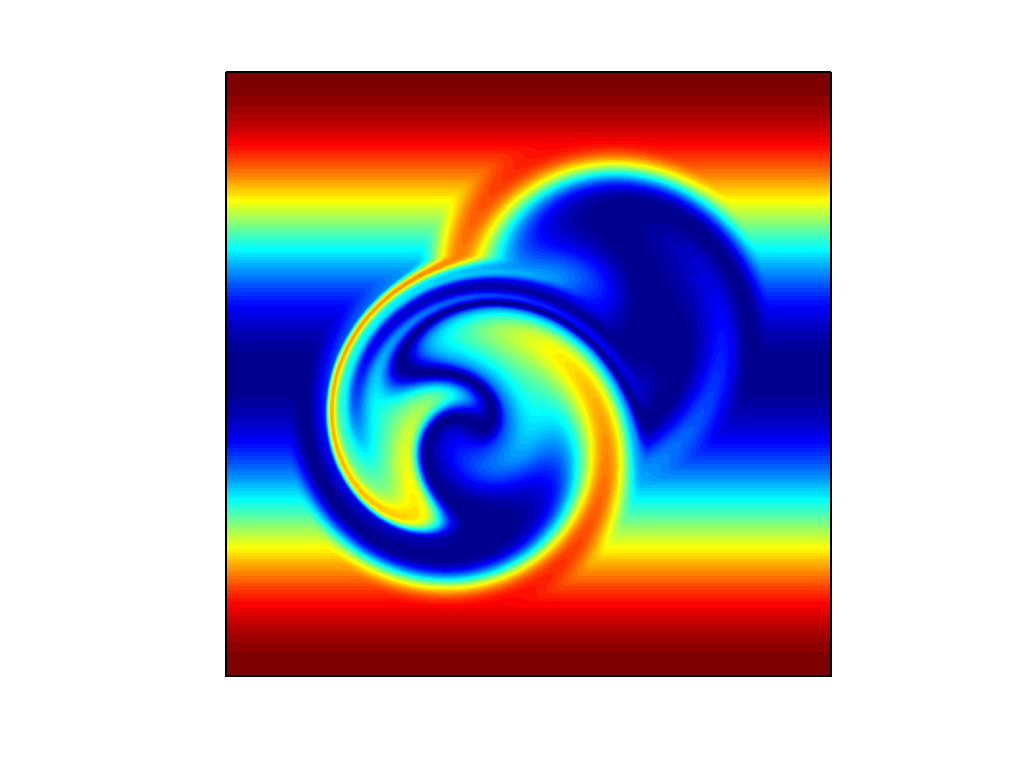
\includegraphics{ltmiter20.eps}}
  \scalebox{0.5}[0.5]{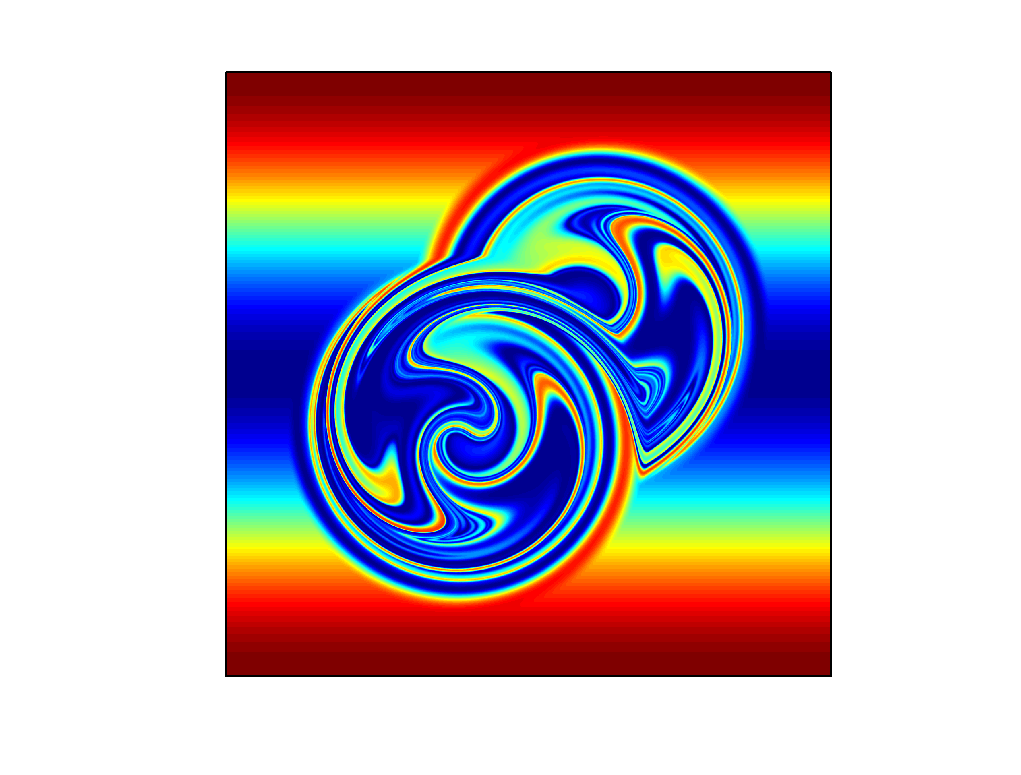
\includegraphics{ltmiter60.eps}}
  }
  \centerline{
  \scalebox{0.5}[0.5]{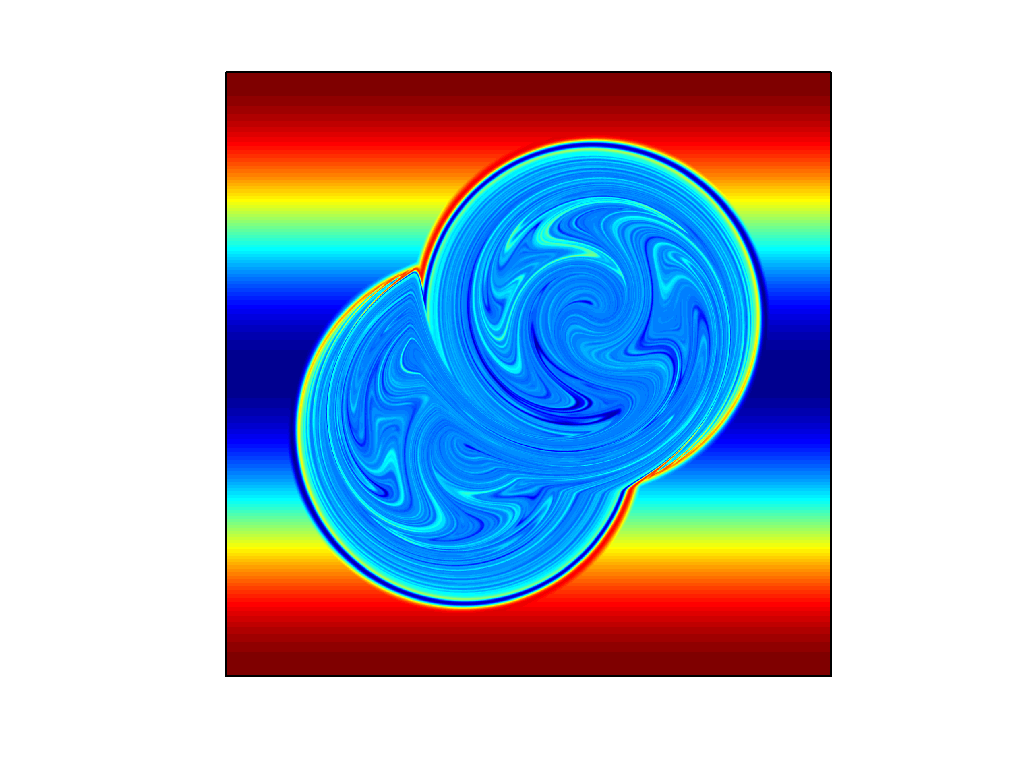
\includegraphics{ltmiter250.eps}}
  \scalebox{0.5}[0.5]{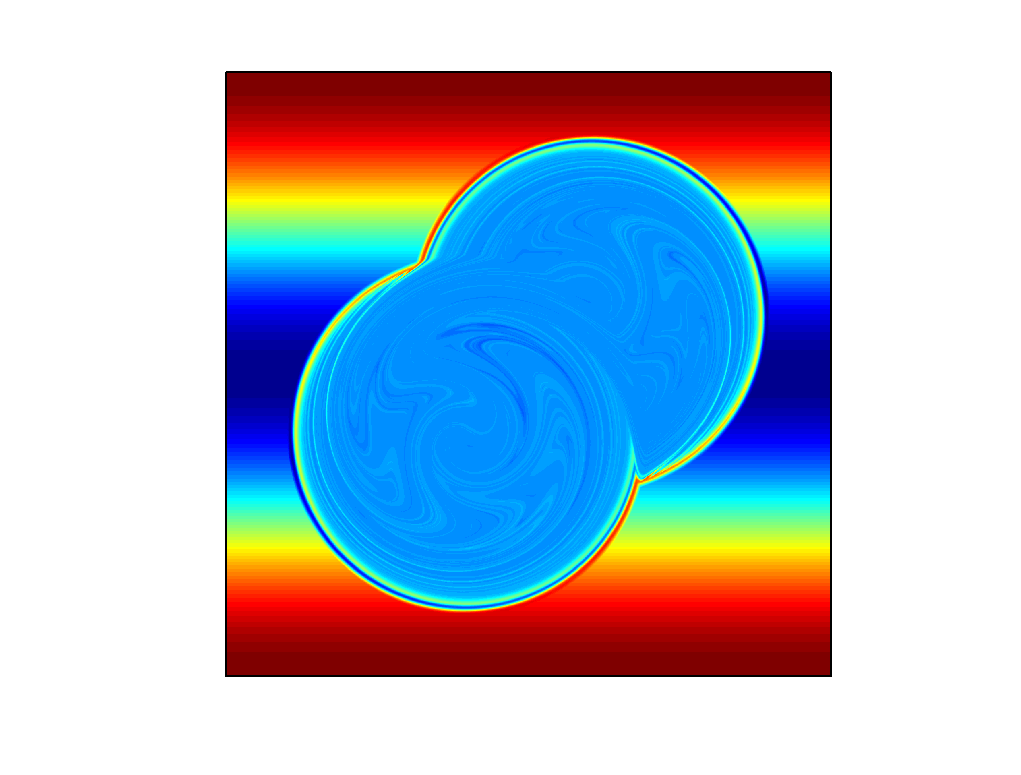
\includegraphics{ltmiter500.eps}}
  }
  \caption{LTM simulations with initial condition $c(x,y)=\cos(y)$,
          (a)iter=20, (b)iter=40, (c)iter=250, (d)=iter=500}
  \label{ltmiter}
\end{figure}


\begin{figure}
 \centerline{
  \scalebox{0.5}[0.5]{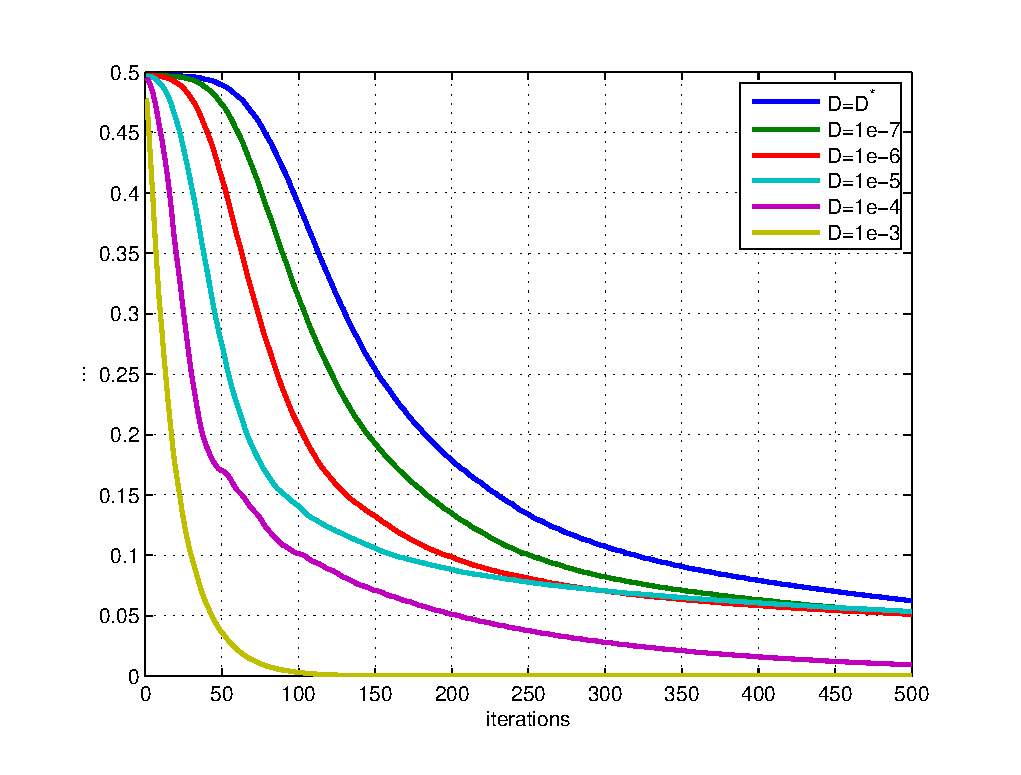
\includegraphics{ltmcutoff.eps}}
  } \caption{LTM}
  \label{democutoff2}
\end{figure}


\end{example}




%%%%%%%%%%%%%%%%%%%%%%%%%%%%%
\section{Remaining Questions}
%%%%%%%%%%%%%%%%%%%%%%%%%%%%%
%%%%%%%%%%%%%%%%%%%%%
\section{Conclusions}
\label{Conclusions}
%%%%%%%%%%%%%%%%%%%%%
\cite{Wiggins2004}
\cite{Ottino2004}
\cite{Mezic2005}
\cite{Thiffeault2003-13}
\cite{Thiffeault2003-309}
\cite{Thiffeault2004}
\cite{Thiffeault2005}
\cite{Ashwin2002}
\cite{Boyd2004}
\cite{Diaconis1996}
\cite{Diaconis2001}
\cite{Diaconis2005}
\cite{Diaconis1986}
\cite{Hammarstr2005}
\cite{Fereday2002}




% References
\bibliographystyle{plain}
\bibliography{mixingbib}

\end{document}
